\documentclass{article}

\usepackage{amsmath, amsthm}
\usepackage{setspace}
\usepackage{microtype, parskip}
\usepackage[comma,sort&compress]{natbib}
\usepackage{lineno}
\usepackage{docmute}
\usepackage{caption, subcaption, multirow, morefloats, rotating}
\usepackage{wrapfig}

\frenchspacing

\doublespacing

\raggedright

\begin{document}
\linenumbers
\modulolinenumbers[2]

%\maketitle

\begin{titlepage}
  \begin{large}
    \textbf{Title:} How do biological traits affect brachiopod taxonomic survival? A hierarchical Bayesian approach.
  \end{large}

  \textbf{Running title:} How do biological traits affect taxonomic survival?

  \textbf{Author:} Peter D Smits, psmits@uchicago.edu, Committee on Evolutionary Biology, University of Chicago

  \textbf{Keywords:} extinction, macroevolution, macroecology, Paleozoic, selection

  \textbf{Word count:} ?
  
  \textbf{Table count:} 0.
 
  \textbf{Figure count:} 5 main text, 3 supplement.

  \textbf{Data archival location:} If accepted, all data and code necessary to duplicate this analysis will be made available on DRYAD.

\end{titlepage}

\begin{abstract}
  While the effect of geographic range on extinction risk is well documented, the effects of other traits are less well known. Using a hierarchical Bayesian modeling approach, I also model the possible interaction between the effects of the biological traits and a taxon's time of origination. I analyze patterns of Paleozoic brachiopod genus durations and their relationship to geographic range, affinity for epicontinental seas versus open ocean environments, and body size. Additionally, I allow for environmental affinity to have a nonlinear effect on duration. My analysis framework eschews the traditional distinction between background and mass extinction, instead the entire time period is analyzed where these ``states'' are part of a continuum. I find evidence that as extinction risk increases, the expected strength of the selection gradient on biological traits (except body size) increases. This manifests as greater expected differences in extinction risk for each unit change in geographic range and environmental preference during periods of high extinction risk, as opposed to a much flatter expected selection gradient during periods of low extinction risk. I find weak evidence for a universally nonlinear relationship between environmental preference and extinction risk such that ``generalists'' have a lower expected extinction risk than either ``specialists''. While for the many parts of the Paleozoic this hypothesis is supported, there are many times where this hypothesized relationship is absent or even reversed. Importantly, I find that as extinction risk increases, the steepness of this relationship is expected to increases as well.
\end{abstract}


\section{Introduction}

How do biological traits affect extinction risk? \citet{Jablonski1986} observed that during periods of high extinction risk, the effects of biological traits on survival decreased in size. However, this pattern was weakest/absent in the effect of geographic range on survival \citep{Jablonski1986}. Biological traits are defined here as descriptors of a taxon's adaptive zone, which is the set of biotic--biotic and biotic--abiotic interactions that a taxon can experience \citep{Simpson1944}. In effect, these are descriptors of a taxon's broad-sense ecology.

\citet{Jablonski1986} phrased his conclusions in terms of background versus mass extinction, but this scenario is readily transferable to a continuous variation framework as there is no obvious distinction in terms of extinction rate between these two states \citep{Wang2003}. Additionally, the \citet{Jablonski1986} scenario has strong model structure requirements in order to test its proposed macroevolutionary mechanism; not only do the taxon trait effects need to be modeled, but the correlation between the trait effects need to be modeled as well. 

There are two end-member macroevolutionary mechanisms which may underlie the pattern observed by \citet{Jablonski1986}: the effect of geographic range on predictive survival remains constant and those of other biological traits decrease, and the effect of geographic range in predicting survival increases and those of other biological traits stay constant. Reality, of course, may fall somewhere along the continuum between these two opposites.

I model brachiopod taxon durations because trait based differences in extinction risk should manifest as differences in taxon durations. Namely, a taxon with a beneficial trait should survive longer, on average, than a taxon without that beneficial trait. Conceptually, taxon survival can be considered an aspect of ``taxon fitness'' along with expected lineage specific branching/origination rate \citep{Cooper1984,Palmer2012}. Brachiopods are an ideal group for this study as they are are well known for having an exceptionally complete fossil records \citep{Foote2000a}. Specifically, I focus on the brachiopod record from most of the Paleozoic, specifically from the start of the Ordovician (approximately 485 Mya) through the end Permian (approximately 252 Mya) as this represents the time of greatest global brachiopod diversity \citep{Alroy2010}.

he analysis of taxon durations, or time from origination to extinction, falls under the purview of survival analysis, a field of applied statistics commonly used in health care \citep{Klein2003} but has a long history in paleontology \citep{Simpson1944,Simpson1953,VanValen1973,VanValen1979}.

Geographic range is widely considered the most important taxon trait for estimating differences in extinction risk at nearly all times with large geographic range associated with low extinction risk \citep{Jablonski1986,Jablonski1987,Jablonski2003,Payne2007}. I expect this to hold true nearly always.

\citet{Miller2009a} demonstrated that during several mass extinctions taxa associated with open-ocean environments tend to have a greater extinction risk than those taxa associated with epicontinental seas. During periods of background extinction, however, they found no consistent difference between taxa favoring either environment. These two environment types represent the primary environmental dichotomy observed in ancient marine systems \citep{Miller2009a,Peters2008,Sheehan2001b}. 

Epicontinental seas are a shallow-marine environment where the ocean has spread over the surface of a continental shelf with a depth typically less than 100m. In contrast, open-ocean coastline environments have much greater variance in depth, do not cover the continental shelf, and can persist during periods of low sea level. Because of this, it is strongly expected that taxa which favor epicontinental seas would be at great risk during periods of low sea levels, such as during glacial periods, where these seas are drained. During the Paleozoic (approximately 541--252 My), epicontinental seas were widely spread globally but declined over the Mesozoic (approximately 252--66 My) and eventually diminished disappearing during the Cenozoic (approximately 66--0 My) as open-ocean coastlines became the dominant shallow-marine setting \citep{Peters2008,Miller2009a,Johnson1974}. 

Given the above information, I predict that as extinction risk increases, taxa associated with open-ocean environments should generally increase in extinction risk versus those that favor epicontinental seas. Additionally, there is a possible nonlinear relationship between environmental preference and taxon duration. A long standing hypothesis is that generalists or unspecialized taxa will have greater survival than specialists \citep{Simpson1944,Liow2004a,Liow2007b,Nurnberg2013a,Nurnberg2015,Baumiller1993}. In this analysis I allowed for environmental preference to possibly have a parabolic effect on taxon duration 

Body size, measured as shell length \citep{Payne2014}, was also considered as a potentially informative covariate. Body size is a proxy for metabolic activity and other correlated life history traits \citep{Payne2014}. There is no strong hypothesis of how body size effects extinction risk in brachiopods, meaning a positive, negative, or zero effect are all plausible. 

I adopt a hierarchical Bayesian survival modeling approach, which represents a conceptual and statistical unification of the paleontological dynamic and cohort survival analytic approaches \citep{VanValen1973,VanValen1979,Raup1978,Raup1975,Foote1988,Baumiller1993,Simpson2006}. By using a Bayesian framework I am able to quantify the uncertainty inherent in the estimates of the effects of biological traits on survival, especially in cases where the covariates of interest (i.e. biological traits) are themselves known with error. 


\section{Materials and Methods}

\subsection{Fossil occurrence information}

The dataset analyzed here was sourced from the Paleobiology Database (http://www.paleodb.org) which was then filtered based on taxonomic, temporal, stratigraphic, and other occurrence information that was necessary for this analysis. These filtering criteria are very similar to those from \citet{Foote2013} with an additional constraint of being present in the body size data set from \citet{Payne2014}. Epicontinental versus open-ocean assignments for each fossil occurrence are partially based on those from \citet{Miller2009a}, with additional occurrences assigned similarly (Miller and Foote, personal communication).

% justification of using genus level versus specific
Fossil occurrences were analyzed at the genus level which is common for paleobiological, macroevolution, or macroecological studies of marine invertebrates \citep{Alroy2010,Foote2013,Harnik2013,Kiessling2007a,Miller2009a,Nurnberg2013a,Nurnberg2015,Payne2007,Simpson2009,Vilhena2013}. While species diversity dynamics are of much greater interest than those of higher taxa, the nature of the fossil record makes accurate and precise taxonomic assignments at the species level for all occurrences. In particular, the simplicity of brachiopod external morphology and the quality of preservation makes it very difficult for assignments below the genus level. As such, the choice to analyze genera as opposed to species was in order to assure a minimum level of confidence and accuracy in the data analyzed here.

Sampled occurrences were restricted to those with paleolatitude and paleolongitude coordinates, assignment to either epicontinental or open-ocean environment, and belonging to a genus present in the body size dataset \citep{Payne2014}. Genus duration was calculated as the number of geologic stages from first appearance to last appearance, inclusive. Durations were based on geologic stages as opposed to millions of years because of the inherently discrete nature of the fossil record; dates are not assigned to fossils themselves but instead fossils are known from a geological interval which represents some temporal range. Stages are effectively irreducible temporal intervals in which taxa may occur.

Genera with a last occurrence in or after Changhsingian stage were right censored at the Changhsingian. Genera with a duration of only one stage were left censored (Appendix \ref{sec:cen}). The covariates used to model genus duration were geographic range size (\(r\)), environmental preference (\(v, v^{2}\)), and body size (\(m\)). 

Geographic range was calculated using an occupancy approach. First, all occurrences were projected onto an equal-area cylindrical map projection. Each occurrence was then assigned to one of the cells from a 70 \(\times\) 34 regular raster grid placed on the map. Each grid cell represents approximately 250,000 km\(^{2}\). The map projection and regular lattice were made using shape files from http://www.naturalearthdata.com/ and the \texttt{raster} package for R \citep{raster}.

For each stage, the total number of occupied grid cells, or cells in which a fossil occurs, was calculated. Then, for each genus, the number of grid cells occupied by that genus was calculated. Dividing the genus occupancy by the total occupancy gives the relative occupancy of that genus. Mean relative genus occupancy was then calculated as the mean of the per stage relative occupancies of that genus. 

Body size data was sourced directly from \citet{Payne2014}. Because those measurements are presented without error, a measurement error model similar to the one for environmental affinity could not be implemented (Appendix \ref{sec:uncer}).

Prior to analysis, geographic range and body size were transformed and standardized in order to improve interpretability of the results. Geographic range, which can only vary between 0 and 1, was logit transformed. Body size, which is defined for all positive real values, was natural log transformed. These covariates were then standardized by mean centering and dividing by two times their standard deviation following \citet{Gelman2007}.

\subsection{Analytical approach}

Hierarchical modelling, sometimes called ``mixed-effects modeling,'' is a statistical approach which explicitly takes into account the structure of the observed data in order to model both the within and between group variance \citep{Gelman2013d,Gelman2007}. The units of study (e.g. genera) each belong to a single grouping (e.g. origination cohort). These groups are considered draws from a shared probability distribution (e.g. all cohorts, observed and unobserved). The group-level parameters are then estimated simultaneously as the other parameters of interest (e.g. covariate effects) \citep{Gelman2013d}. The subsequent estimates are partially pooled together, where parameters from groups with large samples or effects remain large while those of groups with small samples or effects are pulled towards the overall group mean. 

This partial pooling is one of the greatest advantages of hierarchical modeling. By letting the groups ``support'' each other, parameter estimates then better reflect our statistical uncertainty. Additionally, this partial pooling helps control for multiple comparisons and possibly spurious results as effects with little support are drawn towards the overall group mean \citep{Gelman2013d,Gelman2007}. 

All covariate effects (regression coefficients), as well as the intercept term (baseline extinction risk), were allowed to vary by group (origination cohort). The covariance/correlation between covariate effects was also modeled. This hierarchical structure allows inference for how covariates effects may change with respect to each other while simultaneously estimating the effects themselves, propagating our uncertainty through all estimates. 

Additionally, instead of relying on point estimates of environmental affinity, I treat environmental affinity as a continuous measure of the difference between the taxon's environmental occurrence pattern and the background occurrence pattern (Appendix \ref{sec:uncer}).

\subsection{Survival model}

Genus durations were modeled as time-till-event data \citep{Klein2003}, with covariate information used in estimates of extinction risk as a hierarchical regression model. Genus durations were assumed to follow either an exponential or Weibull distribution. THe use of either of these distributions makes assumptions about how duration may effect extinction risk \citep{Klein2003}. The exponential distribution assumes that extinction risk is independent of duration. In contrast, the Weibull distribution allows for age dependent extinction via the shape parameter \(\alpha\), though only as a monotonic function of duration. Importantly, the Weibull distribution is equivalent to the exponential distribution when \(\alpha = 1\). 

The following variables are defined: \(y_{i}\) is the duration of genus \(i\) in geologic stages, \(X\) is the matrix of covariates including a constant term, \(B_{j}\) is the vector of regression coefficients for origination cohort \(j\), \(\Sigma\) is the covariance matrix of the regression coefficients, \(\tau\) is the vector of scales the standard deviations of the between-cohort variation in regression coefficient estimates, and \(\Omega\) is the correlation matrix of the regression coefficients.

The exponential model is defined
\begin{equation}
  \begin{aligned}
    y_{i} &\sim \mathrm{Exponential}(\lambda) \\
    \lambda_{i} &= \exp(\mathbf{X}_{i} B_{j[i]}) \\
    B &\sim \mathrm{MVN}(\vec{\mu}, \Sigma) \\
    \Sigma &= \text{Diag}(\vec{\tau}) \Omega \text{Diag}(\vec{\tau}) \\
    \mu_{k} &\sim 
    \begin{cases} 
      \mathcal{N}(0, \psi_{k} \nu) & \text{if } k \neq r, or \\
      \mathcal{N}(-1, 1) & \text{if } k = r \\
    \end{cases} \\
    \tau_{k} &\sim \mathrm{C^{+}}(1) \\
    \psi_{k} &\sim \mathrm{C^{+}}(1) \text{if } k \neq r \\
    \nu &\sim \mathrm{C^{+}}(1) \\
    \Omega &\sim \text{LKJ}(2).
  \end{aligned}
  \label{eq:exp_total}
\end{equation}

Similarly, the Weibull model is defined
\begin{equation}
  \begin{aligned}
    y_{i} &\sim \mathrm{Weibull}(\alpha, \sigma) \\
    \sigma_{i} &= \exp\left(\frac{-(\mathbf{X}_{i} B_{j[i]})}{\alpha}\right) \\
    B &\sim \mathrm{MVN}(\vec{\mu}, \Sigma) \\
    \Sigma &= \text{Diag}(\vec{\tau}) \Omega \text{Diag}(\vec{\tau}) \\
    \alpha &\sim \mathrm{C^{+}}(2) \\
    \mu_{k} &\sim 
    \begin{cases} 
      \mathcal{N}(0, \psi_{k} \nu) & \text{if } k \neq r, or \\
      \mathcal{N}(-1, 1) & \text{if } k = r \\ 
    \end{cases} \\
    \tau_{k} &\sim \mathrm{C^{+}}(1) \\
    \psi_{k} &\sim \mathrm{C^{+}}(1) \text{if } k \neq r \\
    \nu &\sim \mathrm{C^{+}}(1) \\
    \Omega &\sim \text{LKJ}(2).
  \end{aligned}
  \label{eq:wei_total}
\end{equation}
The principal difference between this model and the previous (Eq. \ref{eq:exp_total}) is the inclusion of the shape parameter \(\alpha\). Note that \(\sigma\) is approximately equivalent to \(1 / \lambda\).

For an explanation of how this model was developed, parameter explanations, and choice of priors, please see Appendix \ref{sec:survival}. Note that these models (Eq. \ref{eq:exp_total}, \ref{eq:wei_total}) do not include how the uncertainty in environmental affinity is included nor how censored observations are included. For an explanation of both of these aspects, see Appendices \ref{sec:uncer} and \ref{sec:cen}.

\subsection{Parameter estimation}

The  joint posterior was approximated using a Markov-chain Monte Carlo routine that is a variant of Hamiltonian Monte Carlo called the No-U-Turn Sampler \citep{Hoffman2014} as implemented in the probabilistic programming language Stan \citep{2014stan}. The posterior distribution was approximated from four parallel chains run for 10,000 draws each, split half warm-up and half sampling and thinned to every 10th sample for a total of 5000 posterior samples. Chain convergence was assessed via the scale reduction factor \(\hat{R}\) where values close to 1 (\(\hat{R} < 1.1\)) indicate approximate convergence. Convergence means that the chains are approximately stationary and the samples are well mixed \citep{Gelman2013d}.

\subsection{Model evaluation}

Models were evaluated using both posterior predictive checks and an estimate of out-of-sample predictive accuracy. The motivation behind posterior predictive checks as tools for determining model adequacy is that replicated data sets using the fitted model should be similar to the original data \citep{Gelman2013d}. Systematic differences between the simulations and observations indicate weaknesses of the model fit. An example of a technique that is very similar would be inspecting the residuals from a linear regression.

The strategy behind posterior predictive checks is to draw simulated values from the joint posterior predictive distribution, \(p(y^{rep} | y)\), and then compare those draws to the empirically observed values \citep{Gelman2013d}. To accomplish this, for each replicate, a single value is drawn from the marginal posterior distributions of each regression coefficient from the final model as well as \(\alpha\) for the Weibull model (Eq. \ref{eq:exp_total}, \ref{eq:wei_total}). Then, given the covariate information \(\mathbf{X}\), a new set of \(n\) genus durations are generated giving a single replicated data set \(y^{rep}\). This is repeated 1000 times in order to provide a distribution of possible values that could have been observed given the model. 

In order to compare the fitted model to the observed data, various graphical comparisons or test quantities need to be defined. The principal comparison used here is a comparison between non-parameteric approximation of the survival function \(S(t)\) as estimated from both the observed data and each of the replicated data sets. The purpose of this comparison is to determine if the model approximates the same survival/extinction pattern as the original data. 

The exponential and Weibull models were compared for out-of-sample predictive accuracy using the widely-applicable information criterion (WAIC) \citep{Watanabe2010a}. Out-of-sample predictive accuracy is a measure of the expected fit of the model to new data. However, because the Weibull model reduces to the exponential model when \(\alpha = 1\) my interest is not in choosing between these models. Instead, comparisons of WAIC values are useful for better understanding the effect of model complexity on out-of-sample predictive accuracy. The calculation of WAIC used here corresponds to the ``WAIC 2'' formulation recommended by \citet{Gelman2013d}. For an explanation of how WAIC is calculated, see Appendix \ref{sec:waic}. Lower values of WAIC indicate greater expected out-of-sample predictive accuracy than higher values.


\section{Results}

As stated above, posterior approximations for both the exponential and Weibull models achieved approximate stationarity after 10,000 steps, as all parameter estimates have an \(\hat{R} < 1.1\).%\uppercase{ref tables}.

Comparisons of the survival functions estimated from 1000 posterior predictive data sets to the estimated survival function of the observed genera demonstrates that both the exponential and Weibull models approximately capture the observed pattern of extinction (Fig. \ref{fig:surv}). The major difference in fit between the two models is that the Weibull model has a slightly better fit for longer lived taxa than the exponential model.

%Inspection of the deviance residuals yields a similar pattern of biased estimates for longer lived taxa \uppercase{ref figure}. 

Additionally, the Weibull model is expected to have slightly better out-of-sample predictive accuracy when compared to the exponential model (WAIC 4576 versus 4604, respectively). \ref{fig:surv}). Because the difference in WAIC between these two models is large, while results from both the exponential and Weibull models will be presented, only those from the Weibull model will be discussed.

% Results/hypothesis tests
%   \mu of hierarchical effects
%   \tau of hierarchical effects (partial pooling)
Estimates of the overall mean covariate effects \(\mu\) can be considered time-invariant generalizations for brachiopod survival during the Paleozoic (Fig. \ref{tab:param}). Consistent with prior expectations, geographic range size has a negative effect on extinction risk, where genera with large ranges having greater durations than genera with small ranges. 

I find that while the mean estimate of the effect of body size on extinction risk is negative, implying that increasing body size decreases extinction risk, this estimate is within 2 standard deviations of 0 (mean \(\mu_{m} = -0.09\), standard deviation 0.09; Fig. \ref{tab:param}). Because of this, I infer that body size has no distinguishable effect on brachiopod taxonomic survival.

Interpretation of the effect of environmental preference \(v\) on duration is slightly more involved. Because a quadratic term is the equivalent of an interaction term, both \(\mu_{v}\) and \(\mu_{v^{2}}\) have to be interpreted together because it is illogical to change values of \(v\) without also changing values \(v^{2}\). To determine the nature of the effect of \(v\) on duration I calculated the multiplicative effect of environmental preference on extinction risk.

Given mean estimated extinction risk \(\tilde{\sigma}\), we can define the extinction risk multiplier of an observation with environmental preference \(v_{i}\) as 
\begin{equation}
  \frac{\tilde{\sigma_{i}}}{\tilde{\sigma}} = f(v_{i}) = \exp\left(\frac{-(\mu_{v} v_{i} + \mu_{v^{2}} v^{2})}{\alpha}\right).
  \label{eq:env}
\end{equation}
This function \(f(v_{i})\) has a y-intercept of \(\exp(0)\) or 1 because it does not have a non-zero intercept term. Equation \ref{eq:env} can be either concave up or down. A concave down \(f(v_{i})\) may indicate that genera of intermediate environmental preference have greater durations than either extreme, and \textit{vice versa} for concave up function.

The expected effect of environmental preference as a multiplier of expected extinction risk can then be visualized (Fig. \ref{fig:env_mean}). This figure depicts 1000 posterior predictive estimates of Eq. \ref{eq:env} across all possible values of \(v\). The number indicates the posterior probability that the function is concave down, with generalists having lower extinction risk/greater duration than either type of specialist. Note that the inflection point/optimum of Fig. \ref{fig:env_mean} is approximately \(x = 0\), something that is expected given the estimate of \(\mu_{v}\) (Fig. \ref{tab:param}).

The matrix \(\Sigma\) describing the covariance between the different coefficients describes how these coefficients might vary together across the origination cohorts. Similar to how this was modeled (Eq. \ref{eq:exp_total}, \ref{eq:wei_total}), for interpretation purposes \(\Sigma\) can be decomposed into a vector of standard deviations \(\vec{\tau}\) and a correlation matrix \(\Omega\).

The estimates of the standard deviation of between-cohort coefficient estimates \(\tau\) inidicate that some effects can vary greatly between-cohorts (Fig. \ref{tab:param}). Coefficients with greater values of \(\tau\) have greater between-cohort variation. The covariate effects with the greatest between origination cohort variation are \(\beta_{r}\), \(\beta_{v}\), and \(\beta_{v^{2}}\). Estimates of \(\beta_{m}\) have negligible between cohort variation, as there is less between cohort variation than the between cohort variation in baseline extinction risk \(\beta_{0}\). However the amount of between cohort variation in estimates of \(\beta_{v^{2}}\) means that it is possible for the function describing the effect of environmental affinity to be upward facing for some cohorts (Eq. \ref{eq:env}), which corresponds to environmental generalists being shorter lived than specialists in that cohort.


% omega heatmap
%   correlations with baseline extinction risk of of major interest
%   high/positive values of intercept --> high extinction risk
%   low/negative values of intercept --> low extinction risk
The correlation terms of \(\Omega\) (Fig. \ref{fig:omega}) describe the relationship between the coefficients and how their estimates may vary together across cohorts. The correlations between the intercept term \(\beta_{0}\) and the effects of the taxon traits are of particular interest for evaluating the \citet{Jablonski1986} scenario (Fig. \ref{fig:omega} first column/last row). Keep in mind that when \(\beta_{0}\) is low, extinction risk is low; and conversely, when \(\beta_{0}\) is high, then extinction risk is high.

Marginal posterior probabilities of the correlations between the level of baseline extinction risk \(\beta_{0}\) and the effects of the taxon traits indicate that the correlation between expected extinction risk and both geographic range \(\beta_{r}\) and \(\beta_{v^{2}}\) are of particular note (Fig. \ref{fig:corr}). 

There is approximately a 98\% probability that \(\beta_{0}\) and \(\beta_{r}\) are negatively correlated (Fig. \ref{fig:corr}), meaning that as extinction risk increases, the effect/importance of geographic range on genus duration increases. This means that increases in baseline extinction rate are correlated with an increased importance of geographic range size. There is a 93\% probability that \(\beta_{0}\) and \(\beta_{v^{2}}\) are negatively correlated (Fig. \ref{fig:corr}), meaning that as extinction risk increases, the peakedness of \(f(v_{i})\) increases and the relationship tends towards concave down. Additionally, there is a 97\% probability that values of \(\beta_{r}\) and \(\beta_{v^{2}}\) are positively correlated (Mean correlation 0.51, standard deviation 0.23).

% effects varying between cohorts
While the overall group level estimates are of particular importance when defining time-invariant differences in extinction risk, it is also important and useful to analyze the individual level parameter estimates in order to better understand how parameters actually vary across cohorts.

In comparison to the overall mean extinction risk \(\mu_{0}\), cohort level estimates \(\beta_{0}\) show some amount of variation through time as expected by estimates of \(\tau_{0}\) (Fig. \ref{fig:cohort_intercept}). A similar, if slightly greater, amount of variation is also observable in cohort estimates of the effect of geographic range \(\beta_{r}\) (Fig. \ref{fig:cohort_range}). Again, smaller values of \(\beta_{0}\) correspond to lower expected extinction risk. Similarly, smaller values of \(\beta_{r}\) correspond to greater decrease in extinction risk with increasing geographic range 

% environmental effect for cohort
%   effect of environmental preference as duration multiplier
How the effect of environmental affinity varies between cohorts can be observed by using the cohort specific coefficients estimates. Following the same procedure used earlier (Fig. \ref{tab:param}), but substituting cohort specific estimates of \(\beta_{v}\) and \(\beta_{v^{2}}\) for \(\mu_{v}\) and \(\mu_{v^{2}}\), the cohort specific effect of environmental preference as a multiplier of mean extinction risk can be calculated. This was done only for the Weibull model, though the observed pattern should be similar for the exponential model. 

As expected based on the estimates of \(\tau_{v}\) and \(\tau_{v^{2}}\), there is greater variation in the peakedness of \(f(v_{i})\) than there is variation between convave up and down functions (Fig. \ref{fig:env_cohort}). 12 of the 33 cohorts have less than 50\% posterior probability that generalists are potentially expected to be shorter lived than specialists, though two of those cases have approximately a 50\% probability of being either concave up or down. This is congruent with the 0.72 posterior probability that \(\mu_{v^{2}}\) is positive/\(f(v_{i})\) is concave down.


Additionally, for some cohorts there is a quite striking pattern where the effect of environmental preference \(v\) has a nearly-linear relationship (Fig. \ref{fig:env_cohort}). These are primarily scenarios where one of the end member preferences is expected to have a greater duration than either intermediate or the opposite end member preference. Whatever curvature is present in these nearly-linear cases is due to the defintion of \(f(v)\) as it is not defined for non-negative values of \(\sigma\) (Eq. \ref{eq:env}). For all stages between the Emsian through the Vis\'{e}an, inclusive, intermediate preferences are of intermediate extinction risk when compared with epicontinental specialists (lowest risk) or open-ocean specialists (highest risk). This time period represents most of the Devonian through the early Carboniferous.


\section{Discussion}

% hypotheses
%   Jablonski1986 hypothesis
My results demonstrate that both the effects of geographic range and the peakedness/concavity of environmental preference are both negatively correlated with baseline extinction risk, meaning that as baseline extinction risk increases the effect sizes of both these traits are expected to increase (Fig. \ref{fig:corr}). This result supports neither of the two proposed macroevolutionary mechanisms for how biological traits should correlate with extinction risk. The observed correlation between the two effects as well as between the effects and baseline extinction risk instead implies that as baseline extinction risk increases, the strength of the total selection gradient on biological traits (except body size) increases. This manifests as greater differences in extinction risk for each unit difference in the biological covariates during periods of high extinction risk, while a relatively flatter selection gradient during periods of low extinction risk.

For the approximately 233 My period analyzed there is an approximate 75\% posterior probability that brachiopod genera with intermediate environmental preferences are expected to have a lower extinction risk than either end members. However, the over all curvature of \(f(v_{i})\) is not very peaked meaning that when averaged over the entire Phanerozoic this relationship may not lead to large differences in extinction risk (Fig. \ref{fig:env_mean}). Note that the duration of the period analyzed is approximately four times then length of the Cenozoic (e.g. time since the extinction of the non-avian dinosaurs). This result gives weak support for the universality of the hypothesis that environmental generalists have greater survival than environmental specialists \citep{Simpson1944,Liow2004a,Liow2007b,Nurnberg2013a,Nurnberg2015}.

The posterior variance in the estimate of overall \(f(v_{i})\) reflects the large between cohort variance in cohort specific estimates of \(f(v_{i})\) (Fig. \ref{fig:env_cohort}). Given that there is only a 75\% posterior probability that the expected overall estimate of \(f(v_{i})\) is concave down, it is not surprising that there are some stages where the estimated relationship is in fact the reverse of the prior expectation. Additionally, some of those same stages where \(f(v_{i})\) does not resemble the prior expectation of a concave down nonlinear relation are instead is highly skewed and effectively linear (Fig. \ref{fig:env_cohort}). These results demonstrate that, while the group-level estimate may only weakly support one hypothesis, the cohort-level estimates may exhibit very different characteristics.These results are also consistent with aspects of \citet{Miller2009a} who found that the effect of environmental preference on extinction risk was quite variable and without obvious patterning during times of background extinction.


%   Miller2009a results
There are two mass extinction events that are captured within the time frame considered here: the Ordovician-Silurian and the Frasnian-Famennian. The cohorts bracketing these events are worth considering in more detail.

% write about the mass extinctions \ref{fig:env_cohort}

The proposed mechanism for the end Ordovician mass extinction is a decrease in sea level and the draining of epicontinental seas due to protracted glaciation \citep{Sheehan2001b,Johnson1974}. My results are broadly consistent with this scenario with both epicontinental and open-ocean specialists having a much lower expected duration than intermediate taxa (Fig. \ref{fig:env_cohort}). All of the stages between the Darriwillian and the Llandovery, except the Hirnantian, have a high probability (90+\%) that \(f(v)\) is concave down. The pattern for the Darriwillian, which proceeds the supposed start of Ordovician glacial activity, demonstrates that taxa tend to favor open-ocean environments are expected to have a greater duration than either intermediate of epicontinental specialists, in decreasing order.

For nearly the entire Devonian estimates of \(f(v)\) indicate that one of the environmental end members is favored over the other end member of intermediate preference (Fig. \ref{fig:env_cohort}). This is consistent with the predictions of \citet{Miller2009a}. For almost the entirely the Givetian though the end of the Devonian and into the Vis\'{e}an, I find that epicontinental favoring taxa are expected to have a greater duration than either intermediate or open-ocean specialists. Additionally, for nearly the entire Devonian and through to the Visean, the cohort-specific estimates of \(f(v)\) are concave-up. This is the opposite pattern than what is expected (Fig. \ref{fig:env_mean}). This result, however, seems to reflect the intensity of the seemingly nearly-linear difference in expected duration across the range of \(v)\) as opposed to an inversion of the weakly expected curvilinear pattern.

% defense
%   species:genus?
%   difficulty towards tails, but that's to be expected
%     this model is about expectations, not tails/extreme events
%     this model is ok for the main part of the data
%     though, of course, this model has a long way to go (all models are false)
Of concern is the use of genera as the unit of the study and how to exactly interpret the effects of the biological traits. For example, if any of the traits analyzed here are associated with increases in speciation rates, this might ``artificially'' increase the duration of genera through self-renewal \citep{Raup1991b,Raup1994}. This could lead to a trait appearing to decrease generic level extinction risk by increasing species level origination rate instead of decreasing species level extinction risk. However, given the nature of the brachiopod fossil record and the difficulty of identifying individual specimens to the species level, there is no simple solution to decreasing this uncertainty in the interpretations of how the biological traits studied here actually affect extinction risk.

% future direction
This model could be improved through either increasing the number of analyzed taxon traits, expanding the hierarchical structure of the model to include other major taxonomic groups of interest, and the inclusion of explicit phylogenetic relationships between the taxa in the model as an additional hierarchical effect.

%   other measures of ecology? affixing strategy a la Alexander1977
An example taxon trait that may be of particular interest is the affixing strategy or method of interaction with the substrate of the taxon. This trait has been found to be related to brachiopod survival \citep{Alexander1977} so its inclusion may be of particular interest.

%   comparison with other major groups in hierarchical model
It is theoretically possible to expand this model to allow for comparisons within and between major taxonomic groups. This approach would better constrain the brachiopod estimates while also allowing for estimation of similarities and differences in cross-taxonomic patterns. The major issue surrounding this particular expansion involves finding an similarly well sampled taxonomic group that is present during the Paleozoic. Example groups include Crinoidea, Ostracoda, and other ``Paleozoic'' groups \citep{SepkoskiJr.1981a}.

%   integration of phylogenetic information/taxonomic component
%     taxon traits are more than likely heritable
%     what aspect of variation is explained just by 
%     see Smits Submitted
Taxon traits like environmental preference or geographic range \citep{Jablonski1987,Hunt2005b} are most likely heritable, at least phylogenetically \citep{Lynch1991,Housworth2004}. Without phylogenetic context, this analysis assumes that differences in extinction risk between taxa are independent of those taxa's shared evolutionary history \citep{Felsenstein1985b}. In contrast, the origination cohorts only capture shared temporal context. The inclusion of phylogenetic context as an addition individual level hierarchical structure independent of origination cohort would allow for determining how much of the observed variability is due to shared evolutionary history versus actual differences associated with these taxonomic traits. 

% concluding statements
In summary, patterns of Paleozoic brachiopod survival were analyzed using a fully Bayesian hierarchical survival modelling approach while also eschewing the traditional separation between background and mass extinction. I modeled both the overall mean effect of biological covariates on extinction risk while also modeling the correlation between cohort-specific estimates of covariate effects. I find that as baseline extinction risk increases, the strength of the selection gradient on biological traits (except body size) increases. This manifests as greater differences in extinction risk for each unit difference in the biological covariates during periods of high extinction risk, while a much flatter total selection gradient during periods of low extinction risk. I also find some support for ``survival of the unspecialized'' \citep{Simpson1944,Liow2004a,Liow2007b,Nurnberg2013a,Nurnberg2015} as a general characterization of the effect of environmental preference on extinction risk (Fig. \ref{fig:env_mean}), though there is heterogeneity between origination cohorts with most periods of time conforming to this hypothesis (Fig. \ref{fig:env_cohort}). 


\section*{Acknowledgements}
I would like to thank K. Angielzcyk, M. Foote, P. D. Polly, and R. Ree for helpful discussion and advice. Additionally, thank you A. Miller for the epicontinental versus open-ocean assignments. This entire study would would not have been possible without the Herculean effort of the many contributors to the Paleobiology Database. In particular, I would like to thank J. Alroy, M. Aberhan, D. Bottjer, M. Clapham, F. F\"{u}rsich, N. Heim, A. Hendy, S. Holland, L. Ivany, W. Kiessling, B. Kr\"{o}ger, A. McGowan, T. Olszewski, P. Novack-Gottshall, M. Patzkowsky, M. Uhen, L. Villier, and P. Wager. This work was supported by a NASA Exobiology grant (NNX10AQ446) to A. Miller and M. Foote. This is Paleobiology Database publication XXX.

\clearpage

\bibliographystyle{evolution}
\bibliography{newbib,packages}

\clearpage

\begin{figure}[ht]
  \centering
  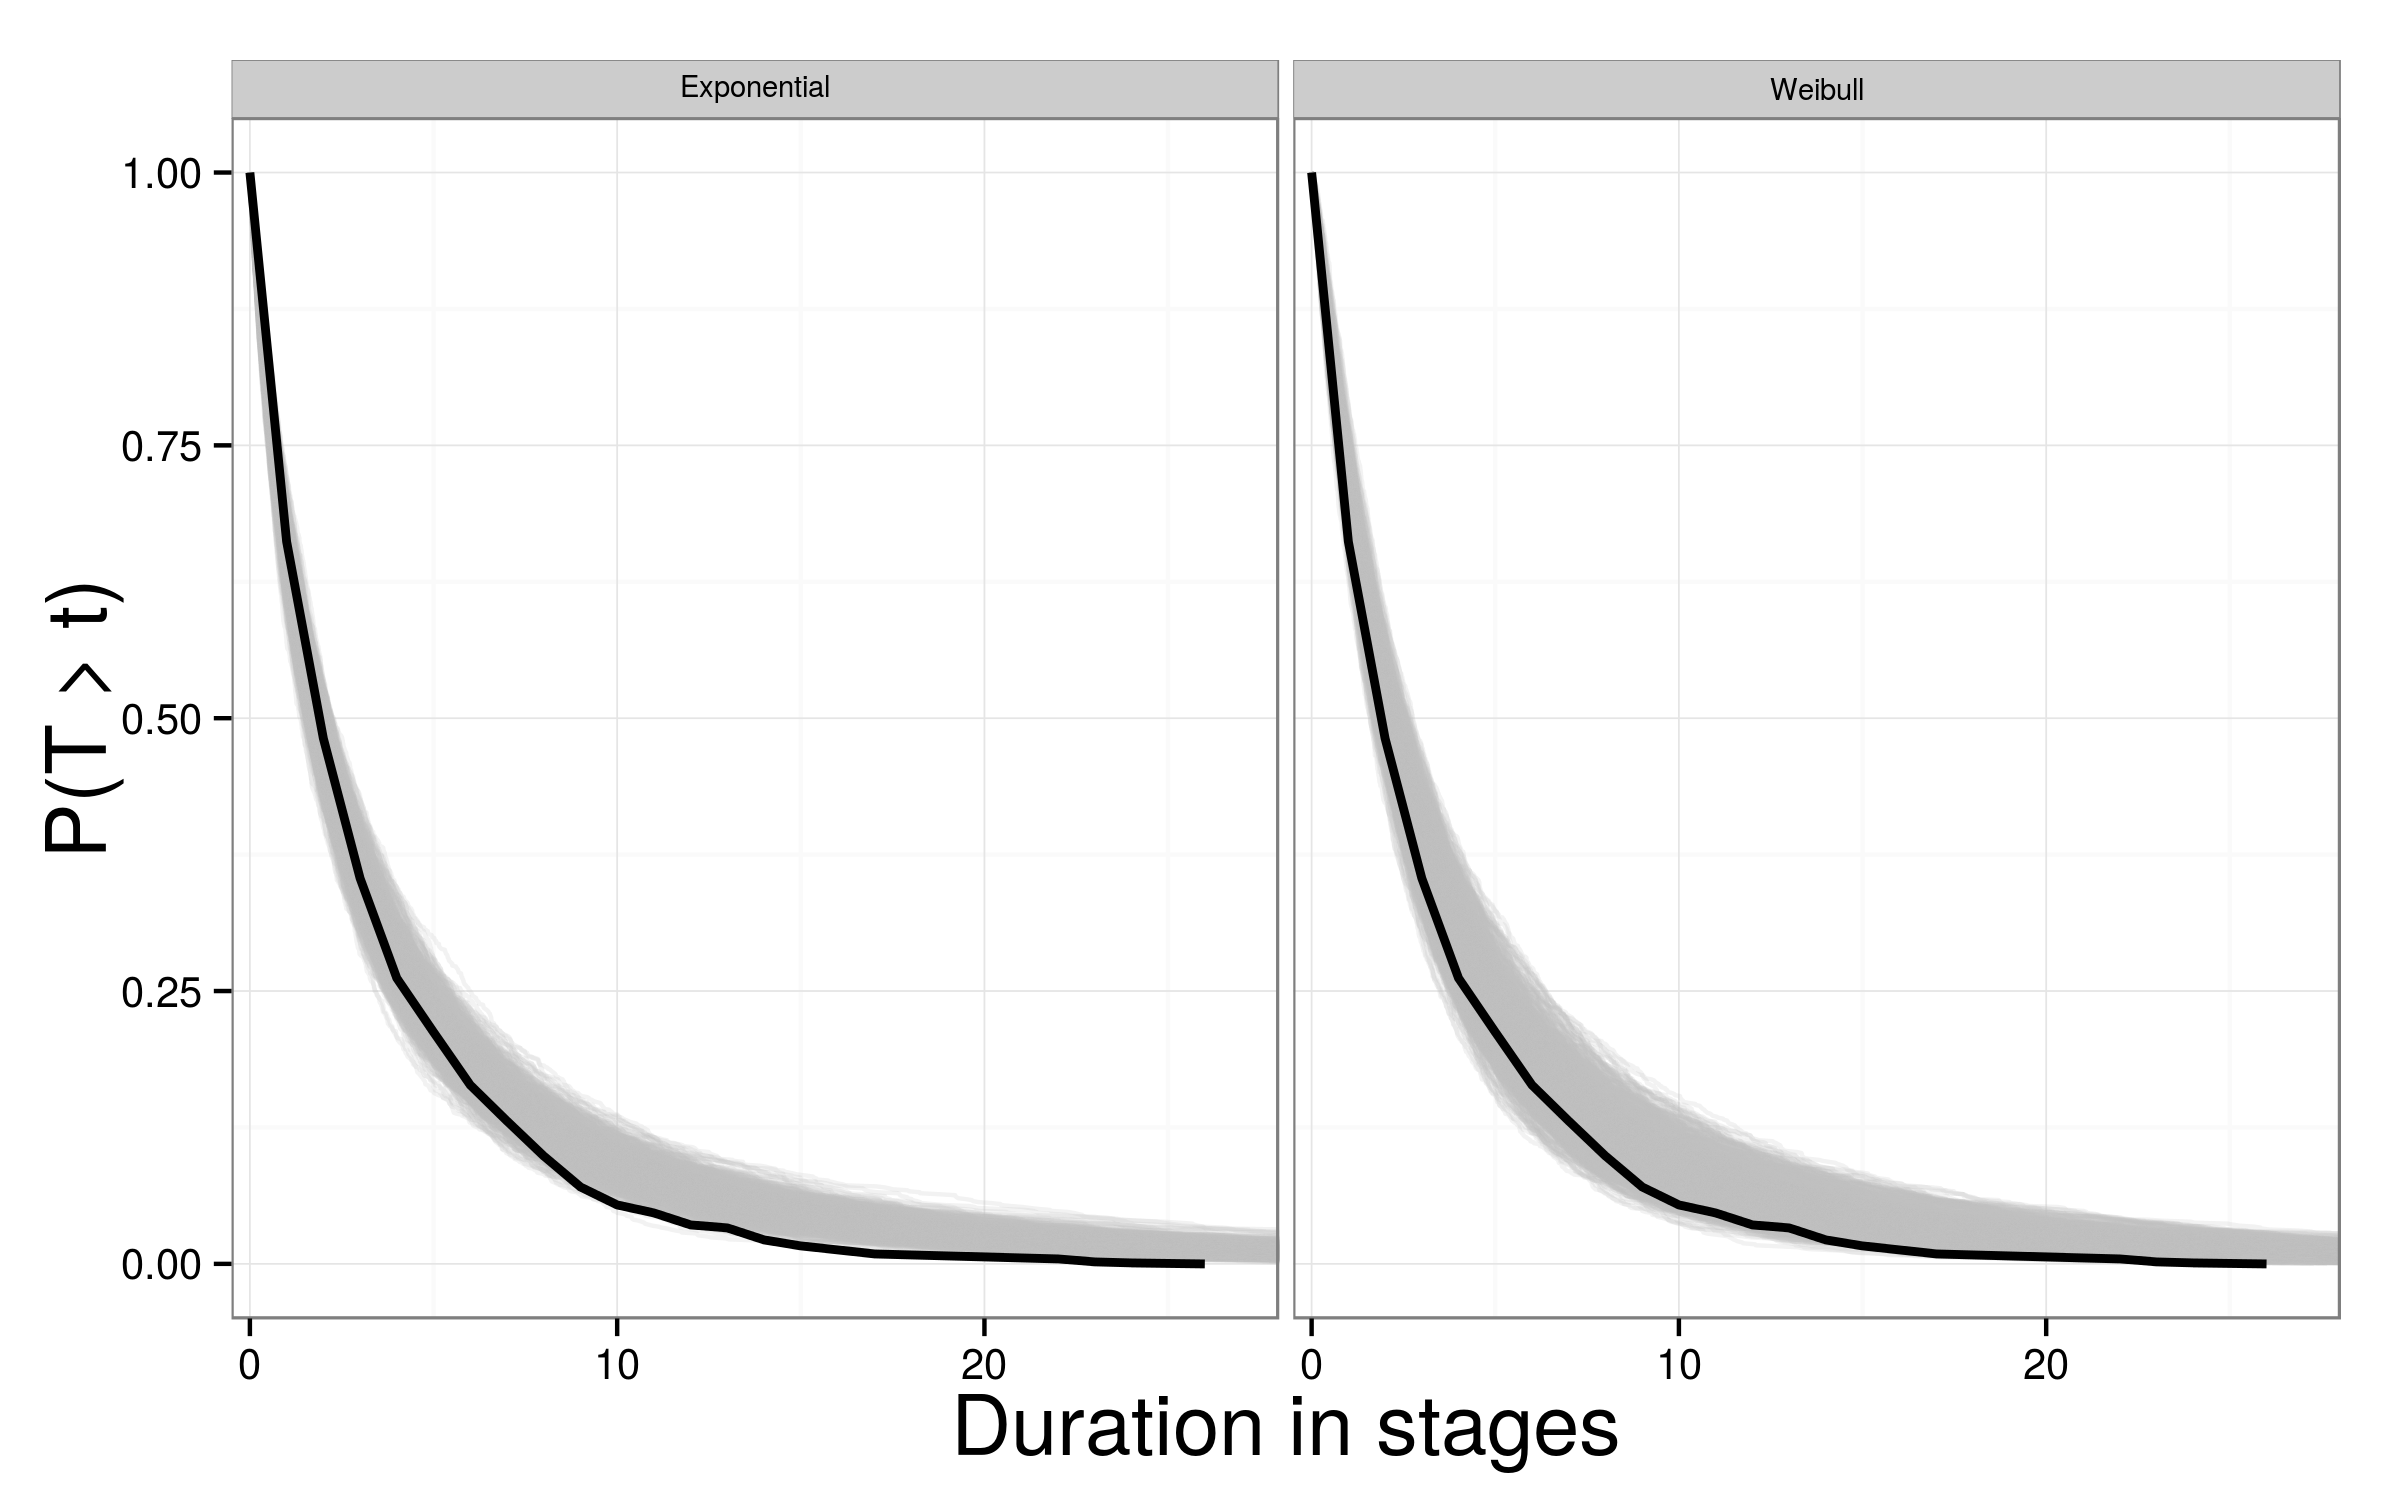
\includegraphics[height = 0.5\textheight,width=\textwidth,keepaspectratio=true]{figure/survival_curves}
  \caption{Comparison of empirical estimates of \(S(t)\) versus estimates from 1000 posterior predictive data sets. \(S(t)\) corresponds to \(P(T > t)\) as it is the probability that a given genus observed at age \(t\) will continue to live. This is equivalent to the probability that \(t\) is less than the genus' ultimate duration \(T\). Note that the Weibull (left) model has noticeably better fit to the data than the exponential (right).}
  \label{fig:surv}
\end{figure}

\begin{figure}[ht]
  \centering
  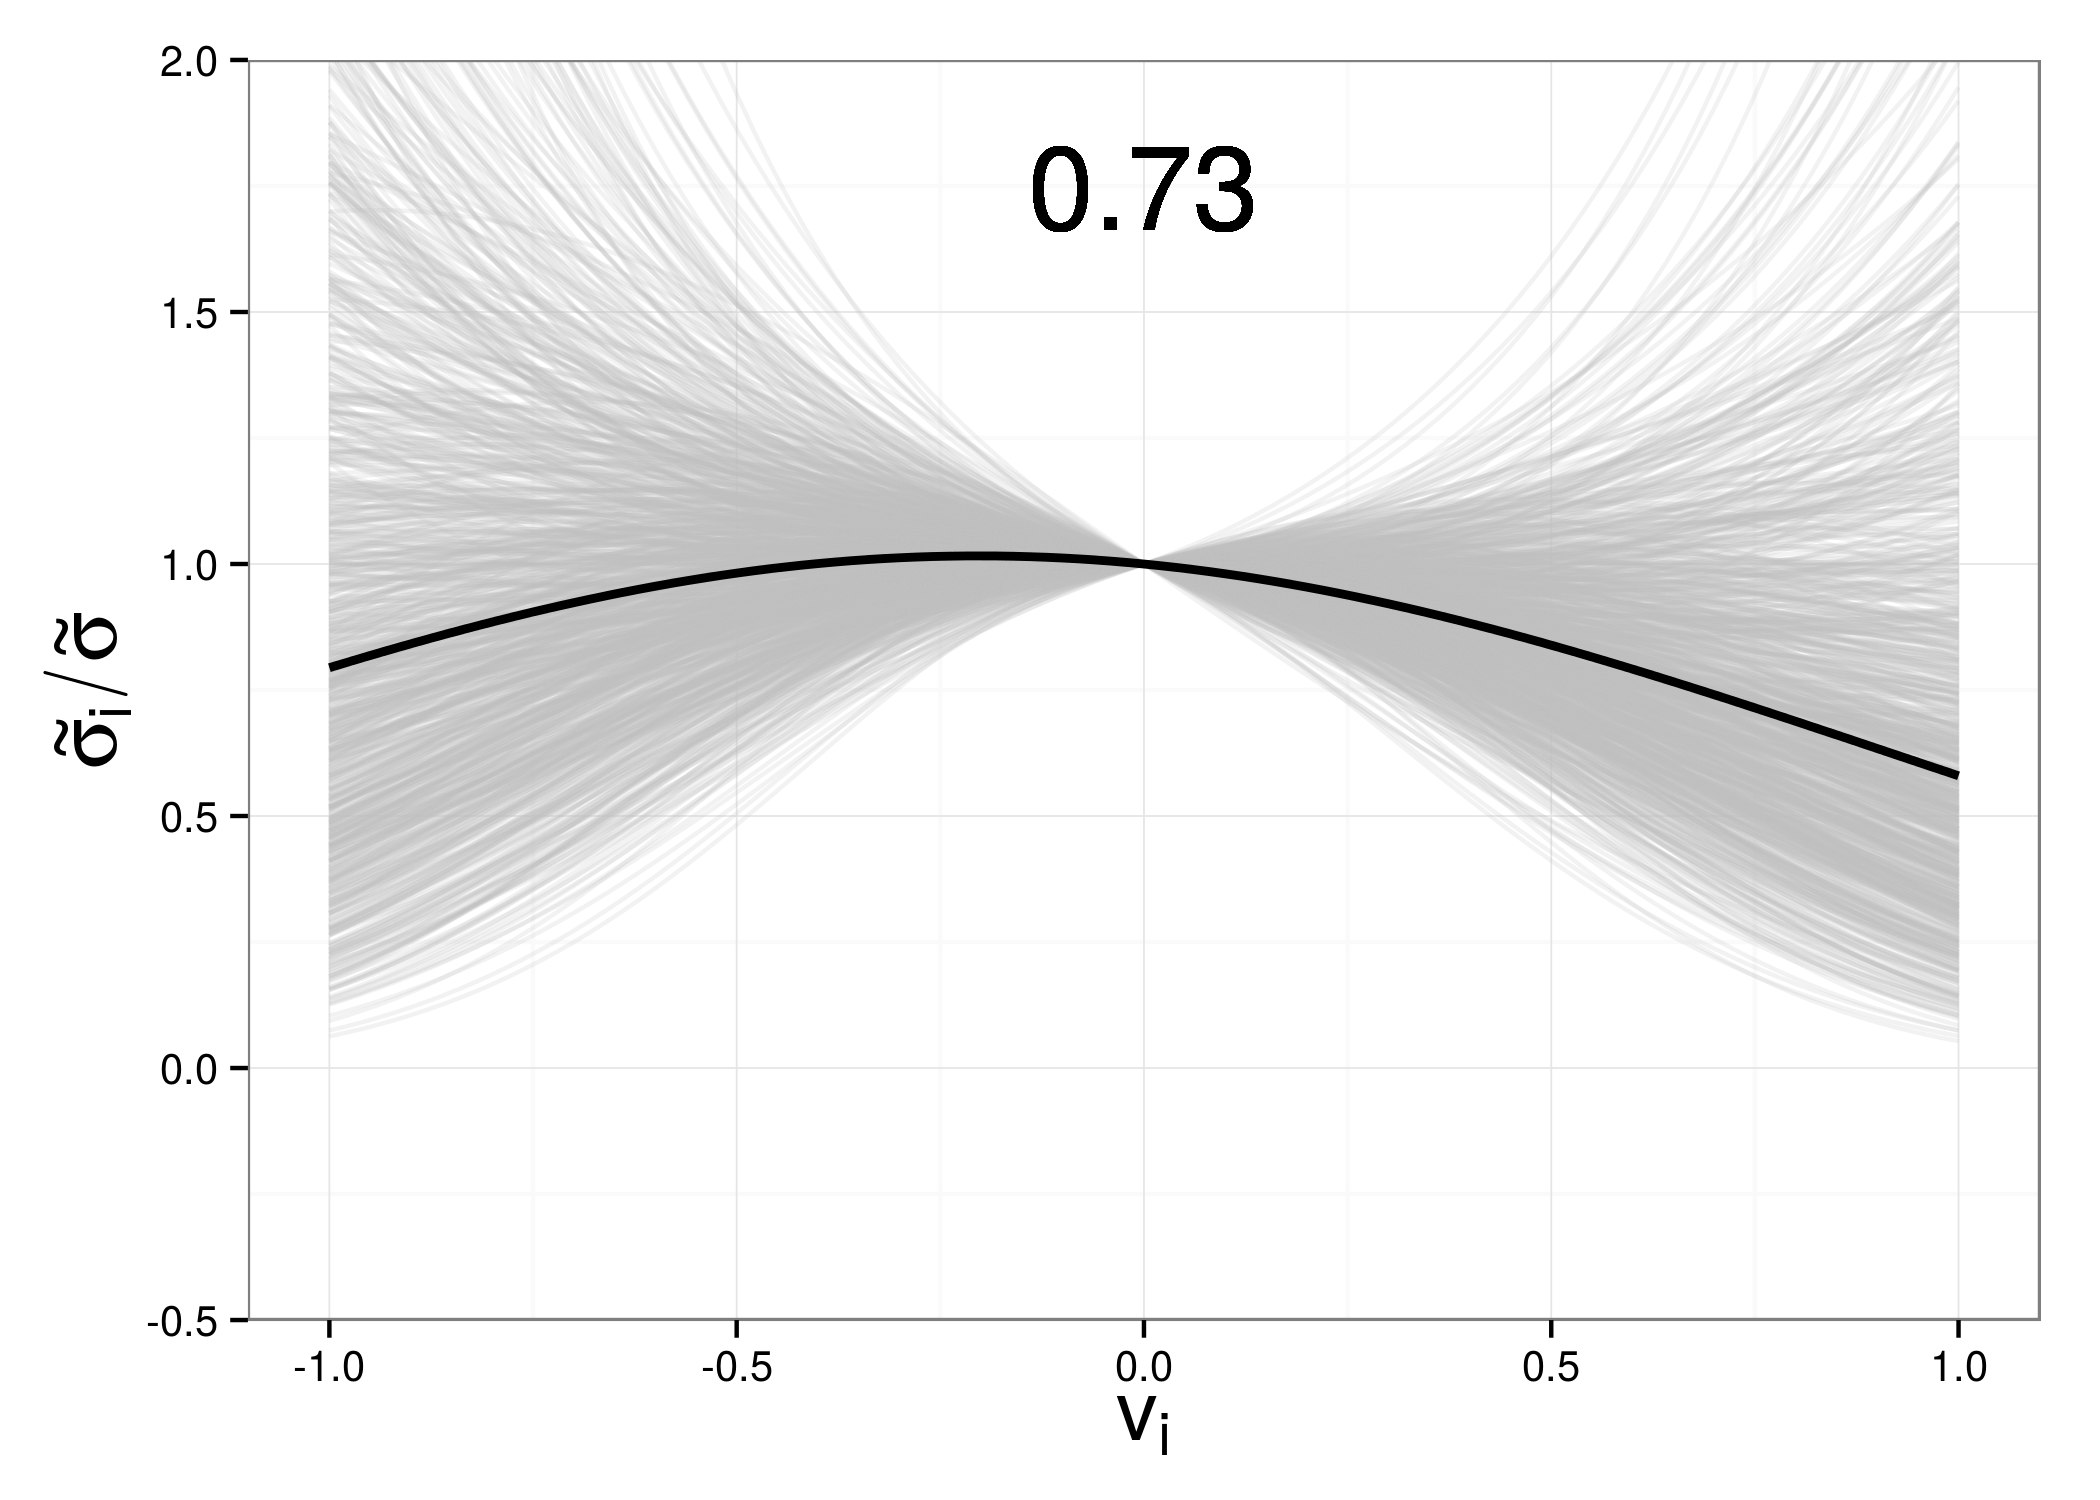
\includegraphics[height = 0.5\textheight,width=\textwidth,keepaspectratio=true]{figure/environ_quad}
  \caption{The overall expected relationship \(f(v_{i})\) between environmental affinity \(v_{i}\) and a multiplier of extinction risk (Eq. \ref{eq:env}). Each grey line corresponds to a single draw from the posterior predictive distribution, while the black corresponds to the median of the posterior predictive distribution. The overall shape of \(f(v_{i})\) is concave down with an optimum of close 0, which corresponds to affinity approximately equal to the expectation based on background environmental occurrence rates.}
  \label{fig:env_mean}
\end{figure}


\begin{figure}[ht]
  \centering
  \begin{subfigure}[b]{0.5\textwidth}
    \caption{}
    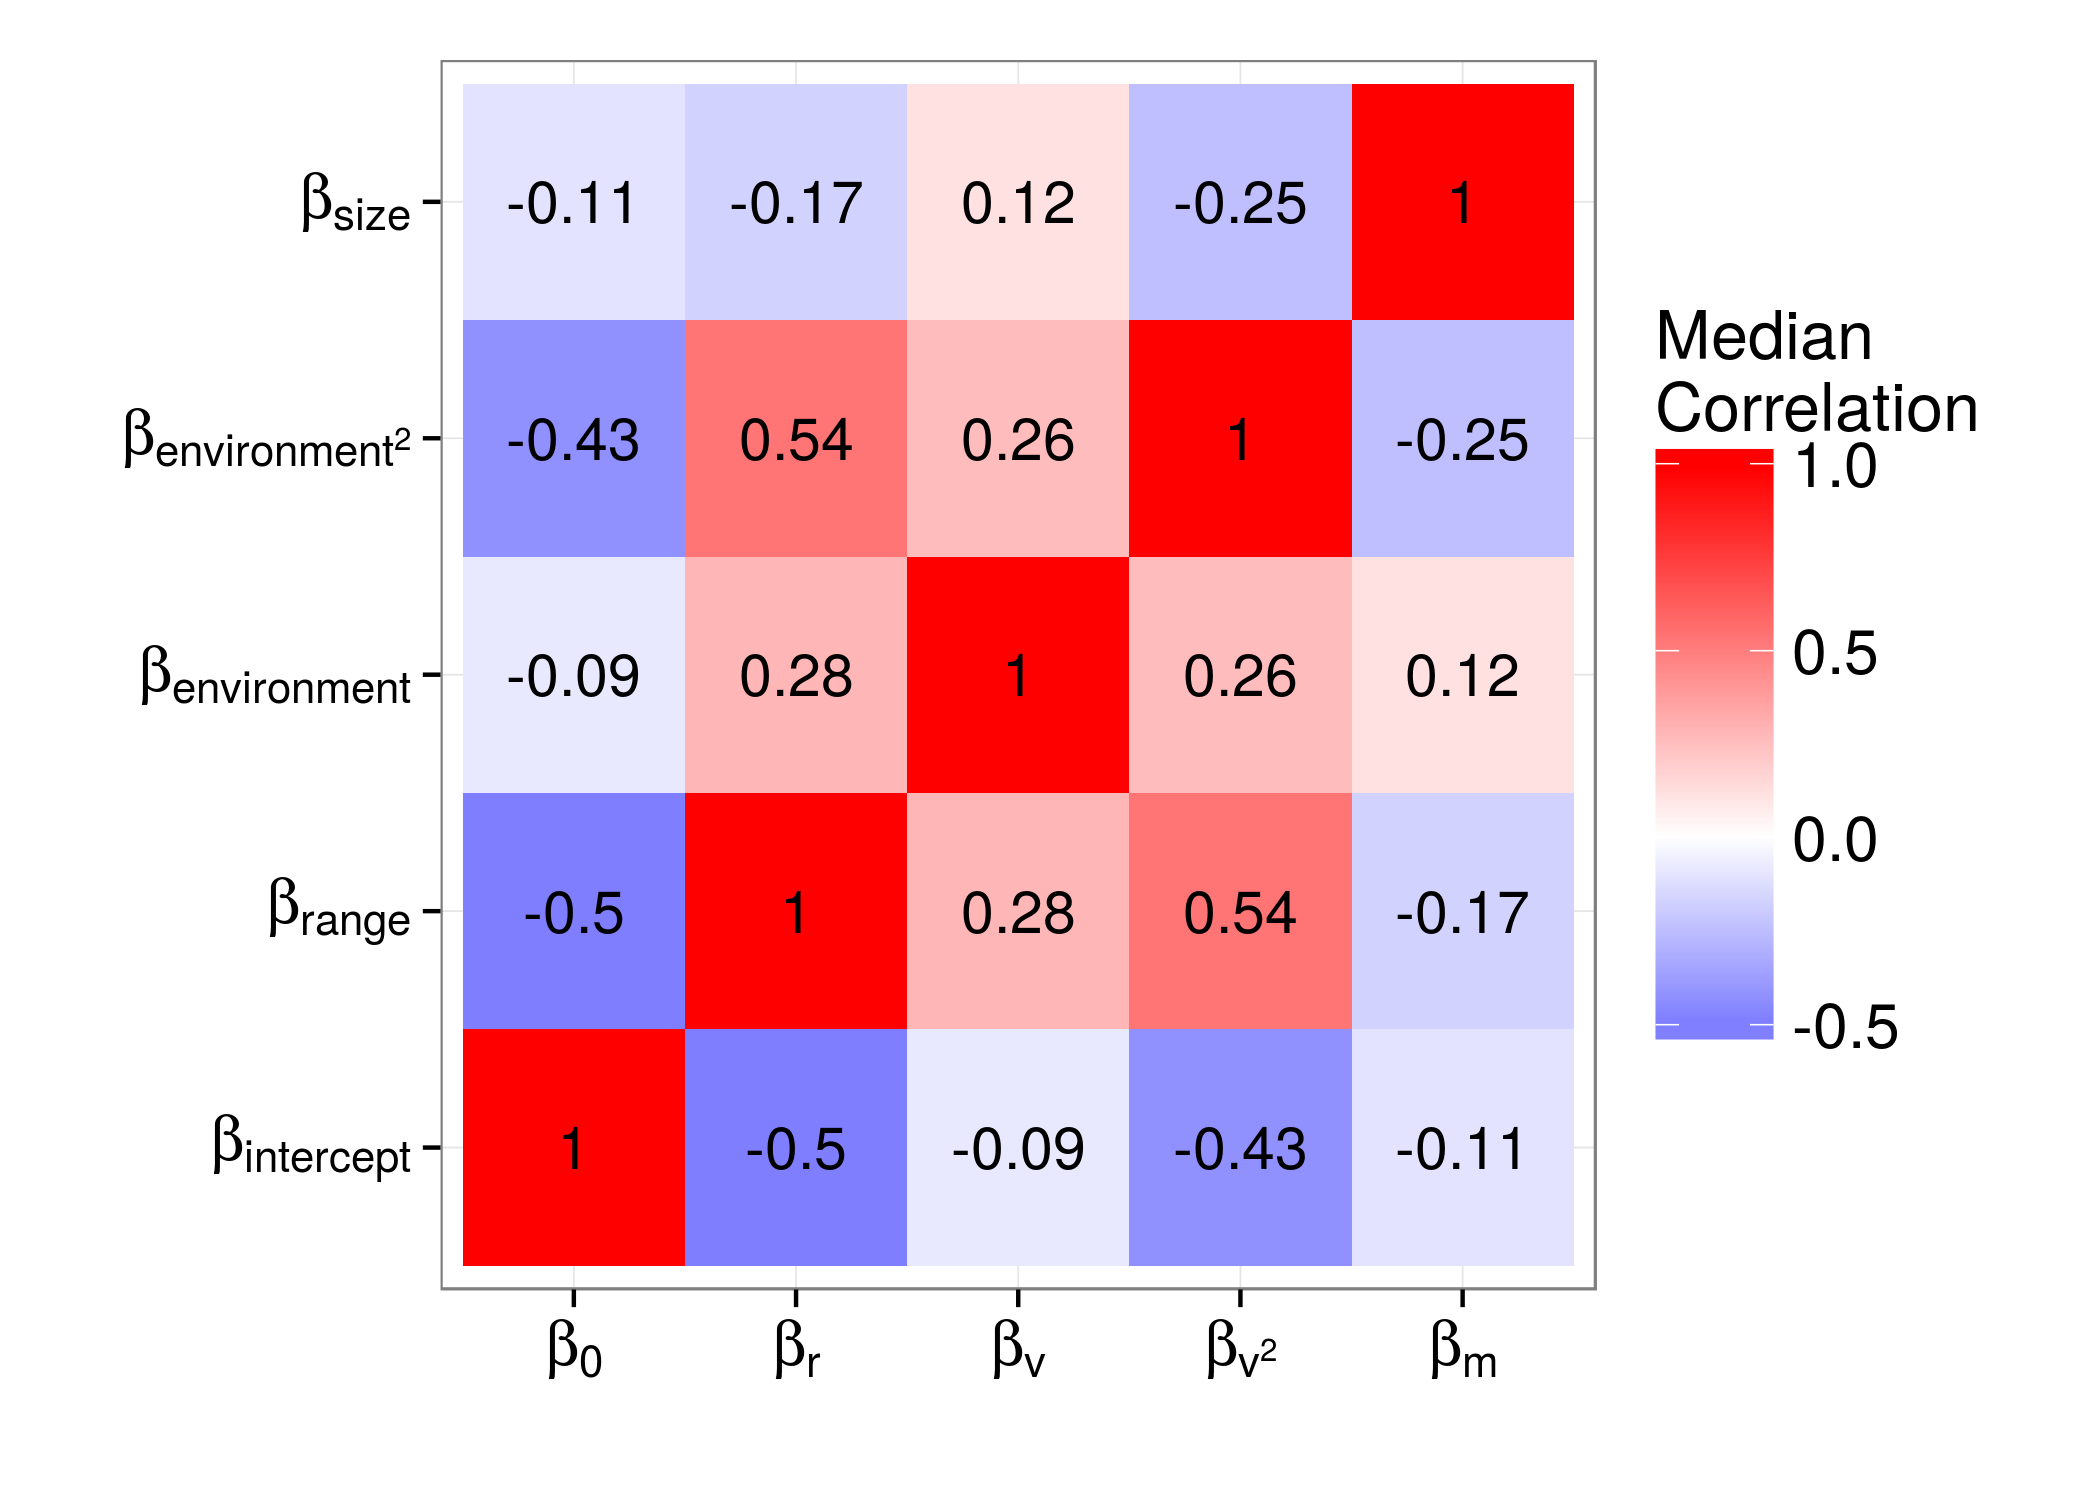
\includegraphics[height = 0.5\textheight,width=\textwidth,keepaspectratio=true]{figure/wei_cor_heatmap}
    \label{fig:omega}
  \end{subfigure}
  \begin{subfigure}[b]{0.4\textwidth}
    \caption{}
    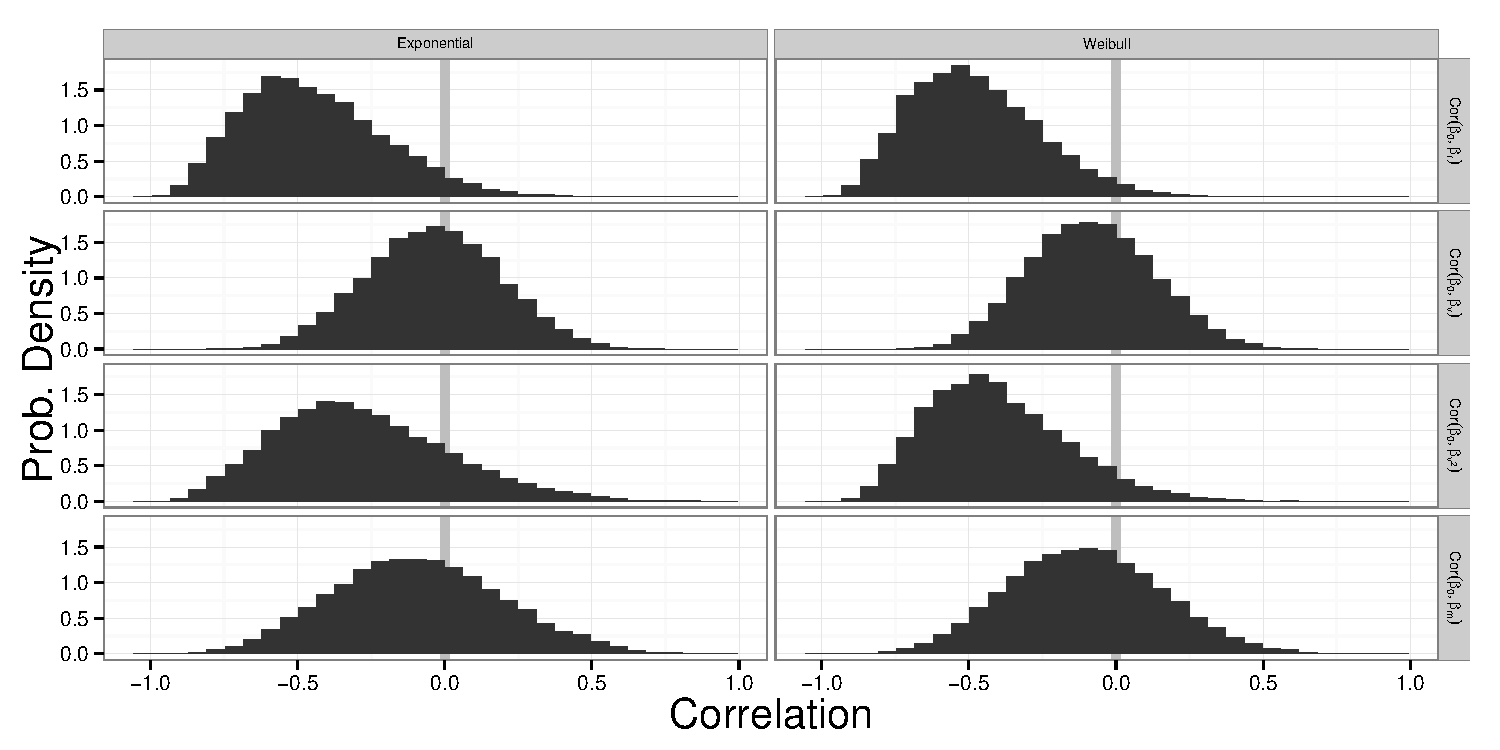
\includegraphics[height = 0.5\textheight,width=\textwidth,keepaspectratio=true]{figure/correlation_marginal}
    \label{fig:corr}
  \end{subfigure}
  \caption{\textbf{A}: Heatmap for the median estimates of the terms of the correlation matrix \(\Omega\) between cohort-level covariate effects. Both the exponential (left) and Weibull (right) models are presented. The off-diagonal terms are the correlation between the estimates of the cohort-level estimates of the effects of covariates, along with intercept/baseline extinction risk. \textbf{B}: Marginal posterior distributions of the correlations between intercept terms/baseline extinction risk and the effects of each of the covariates. These are presented for both the exponential (left) and Weibull (right) models.}
  \label{fig:cor_posterior}
\end{figure}


\begin{figure}[ht]
  \centering
  \begin{subfigure}[b]{\textwidth}
    \caption{}
    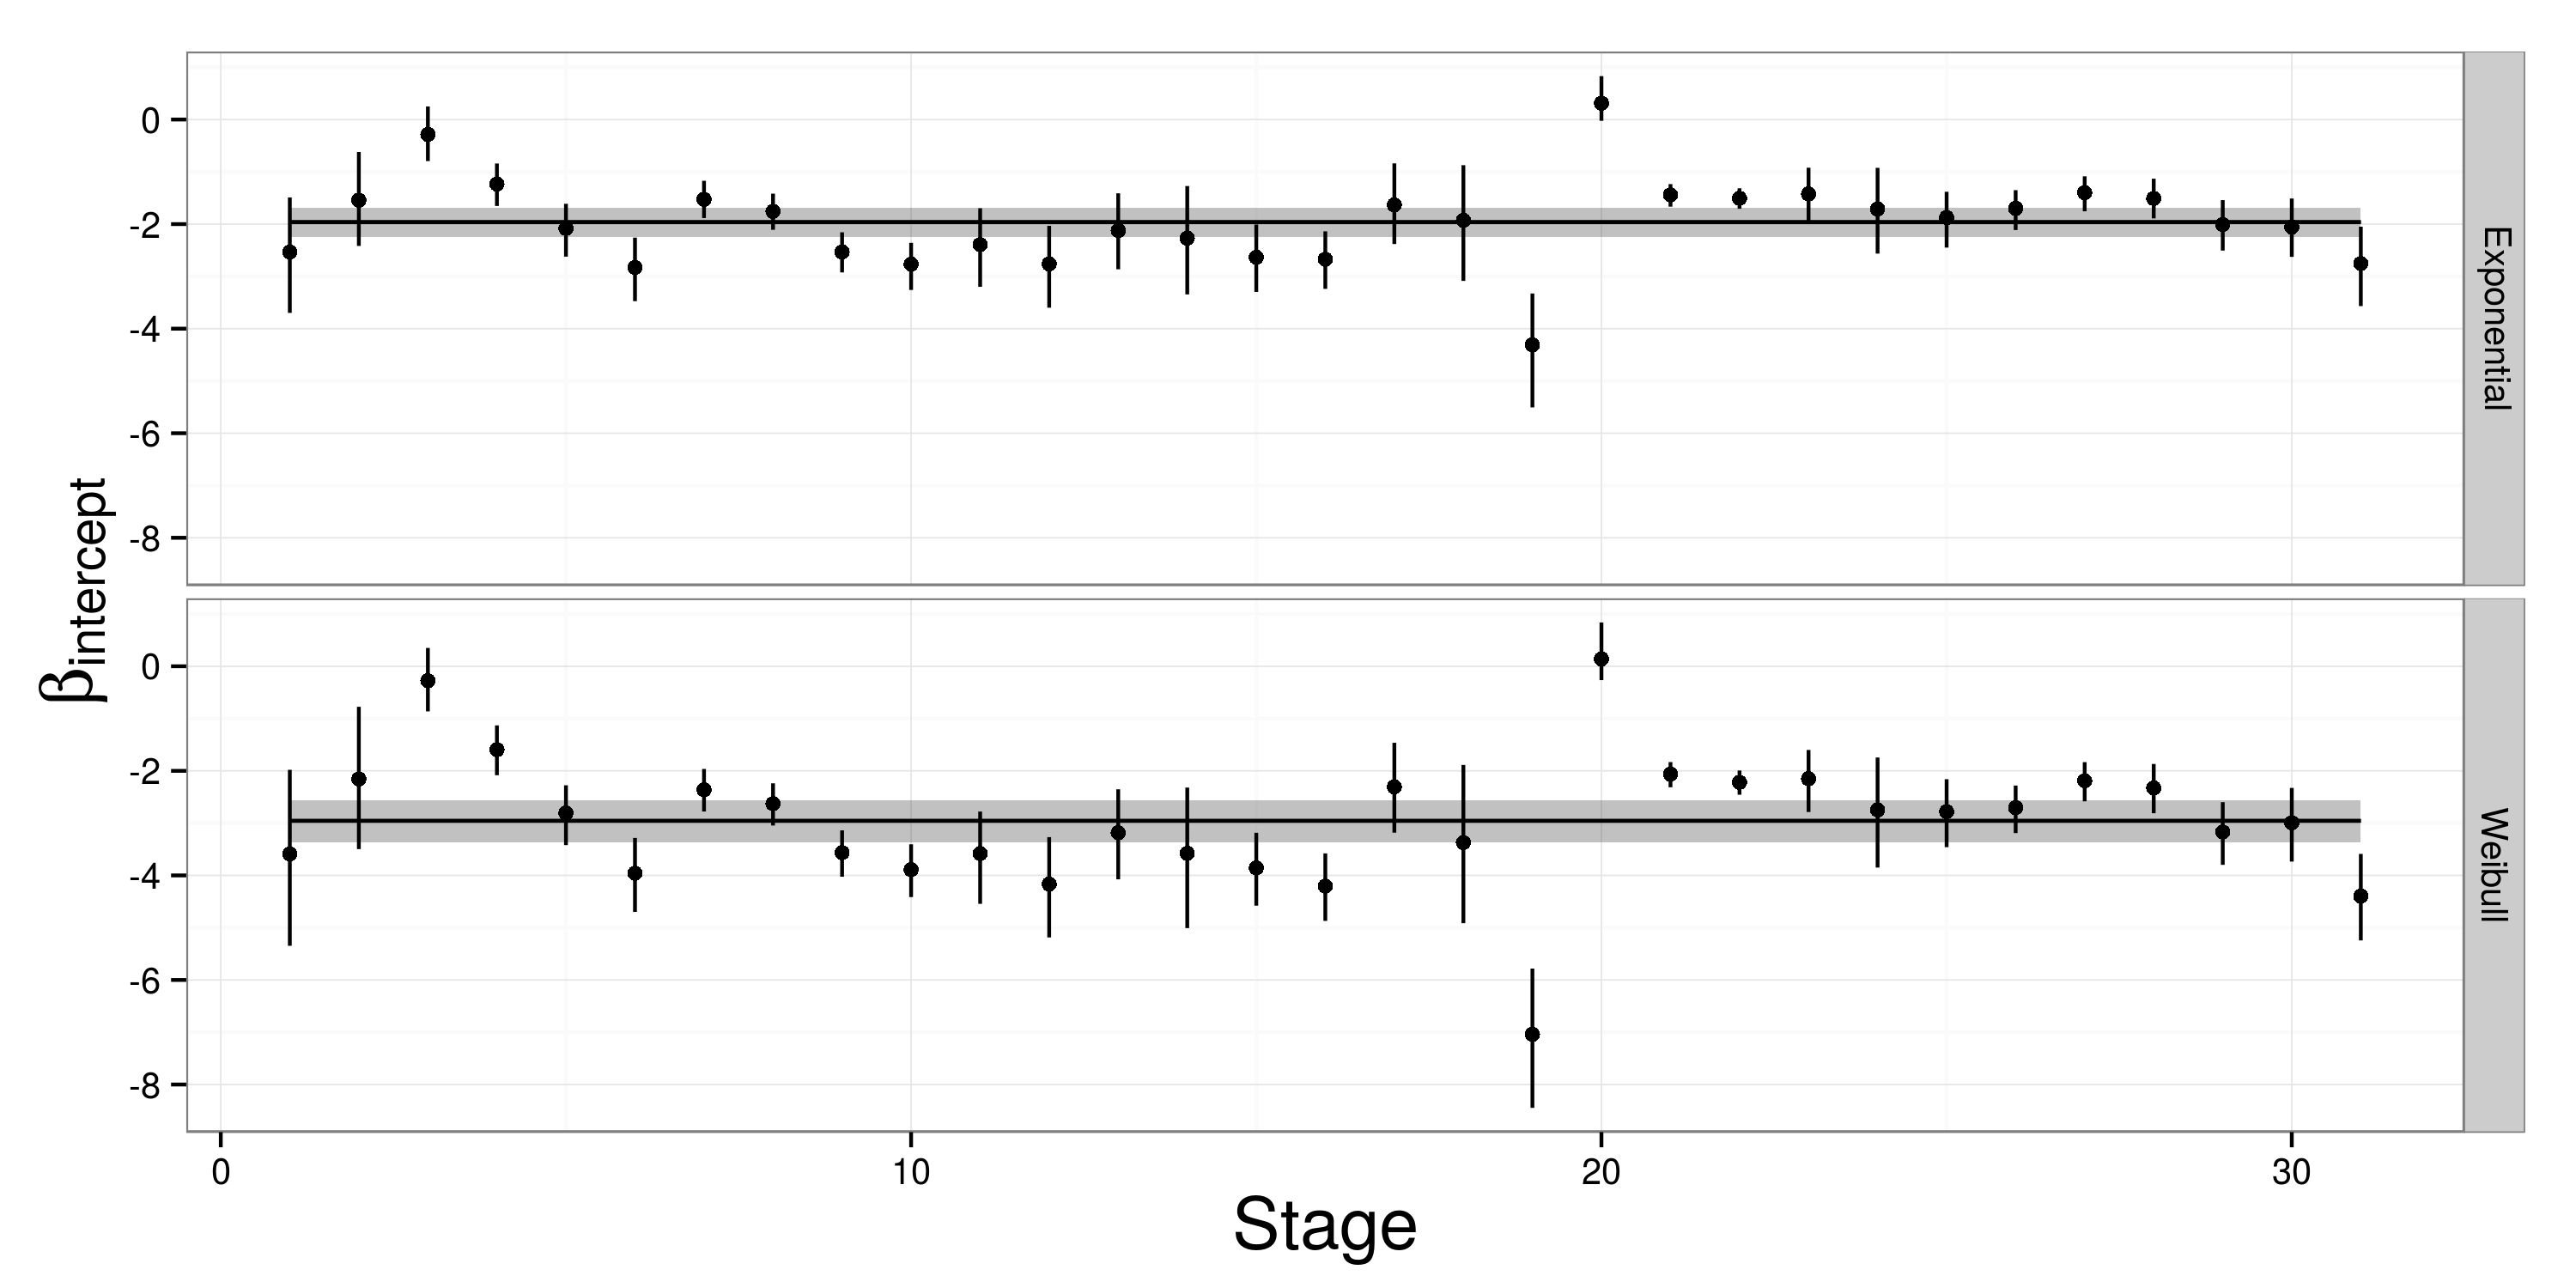
\includegraphics[width = \textwidth,keepaspectratio=true]{figure/intercept_cohort}
    \label{fig:cohort_intercept}
  \end{subfigure}

  \begin{subfigure}[b]{\textwidth}
    \caption{}
    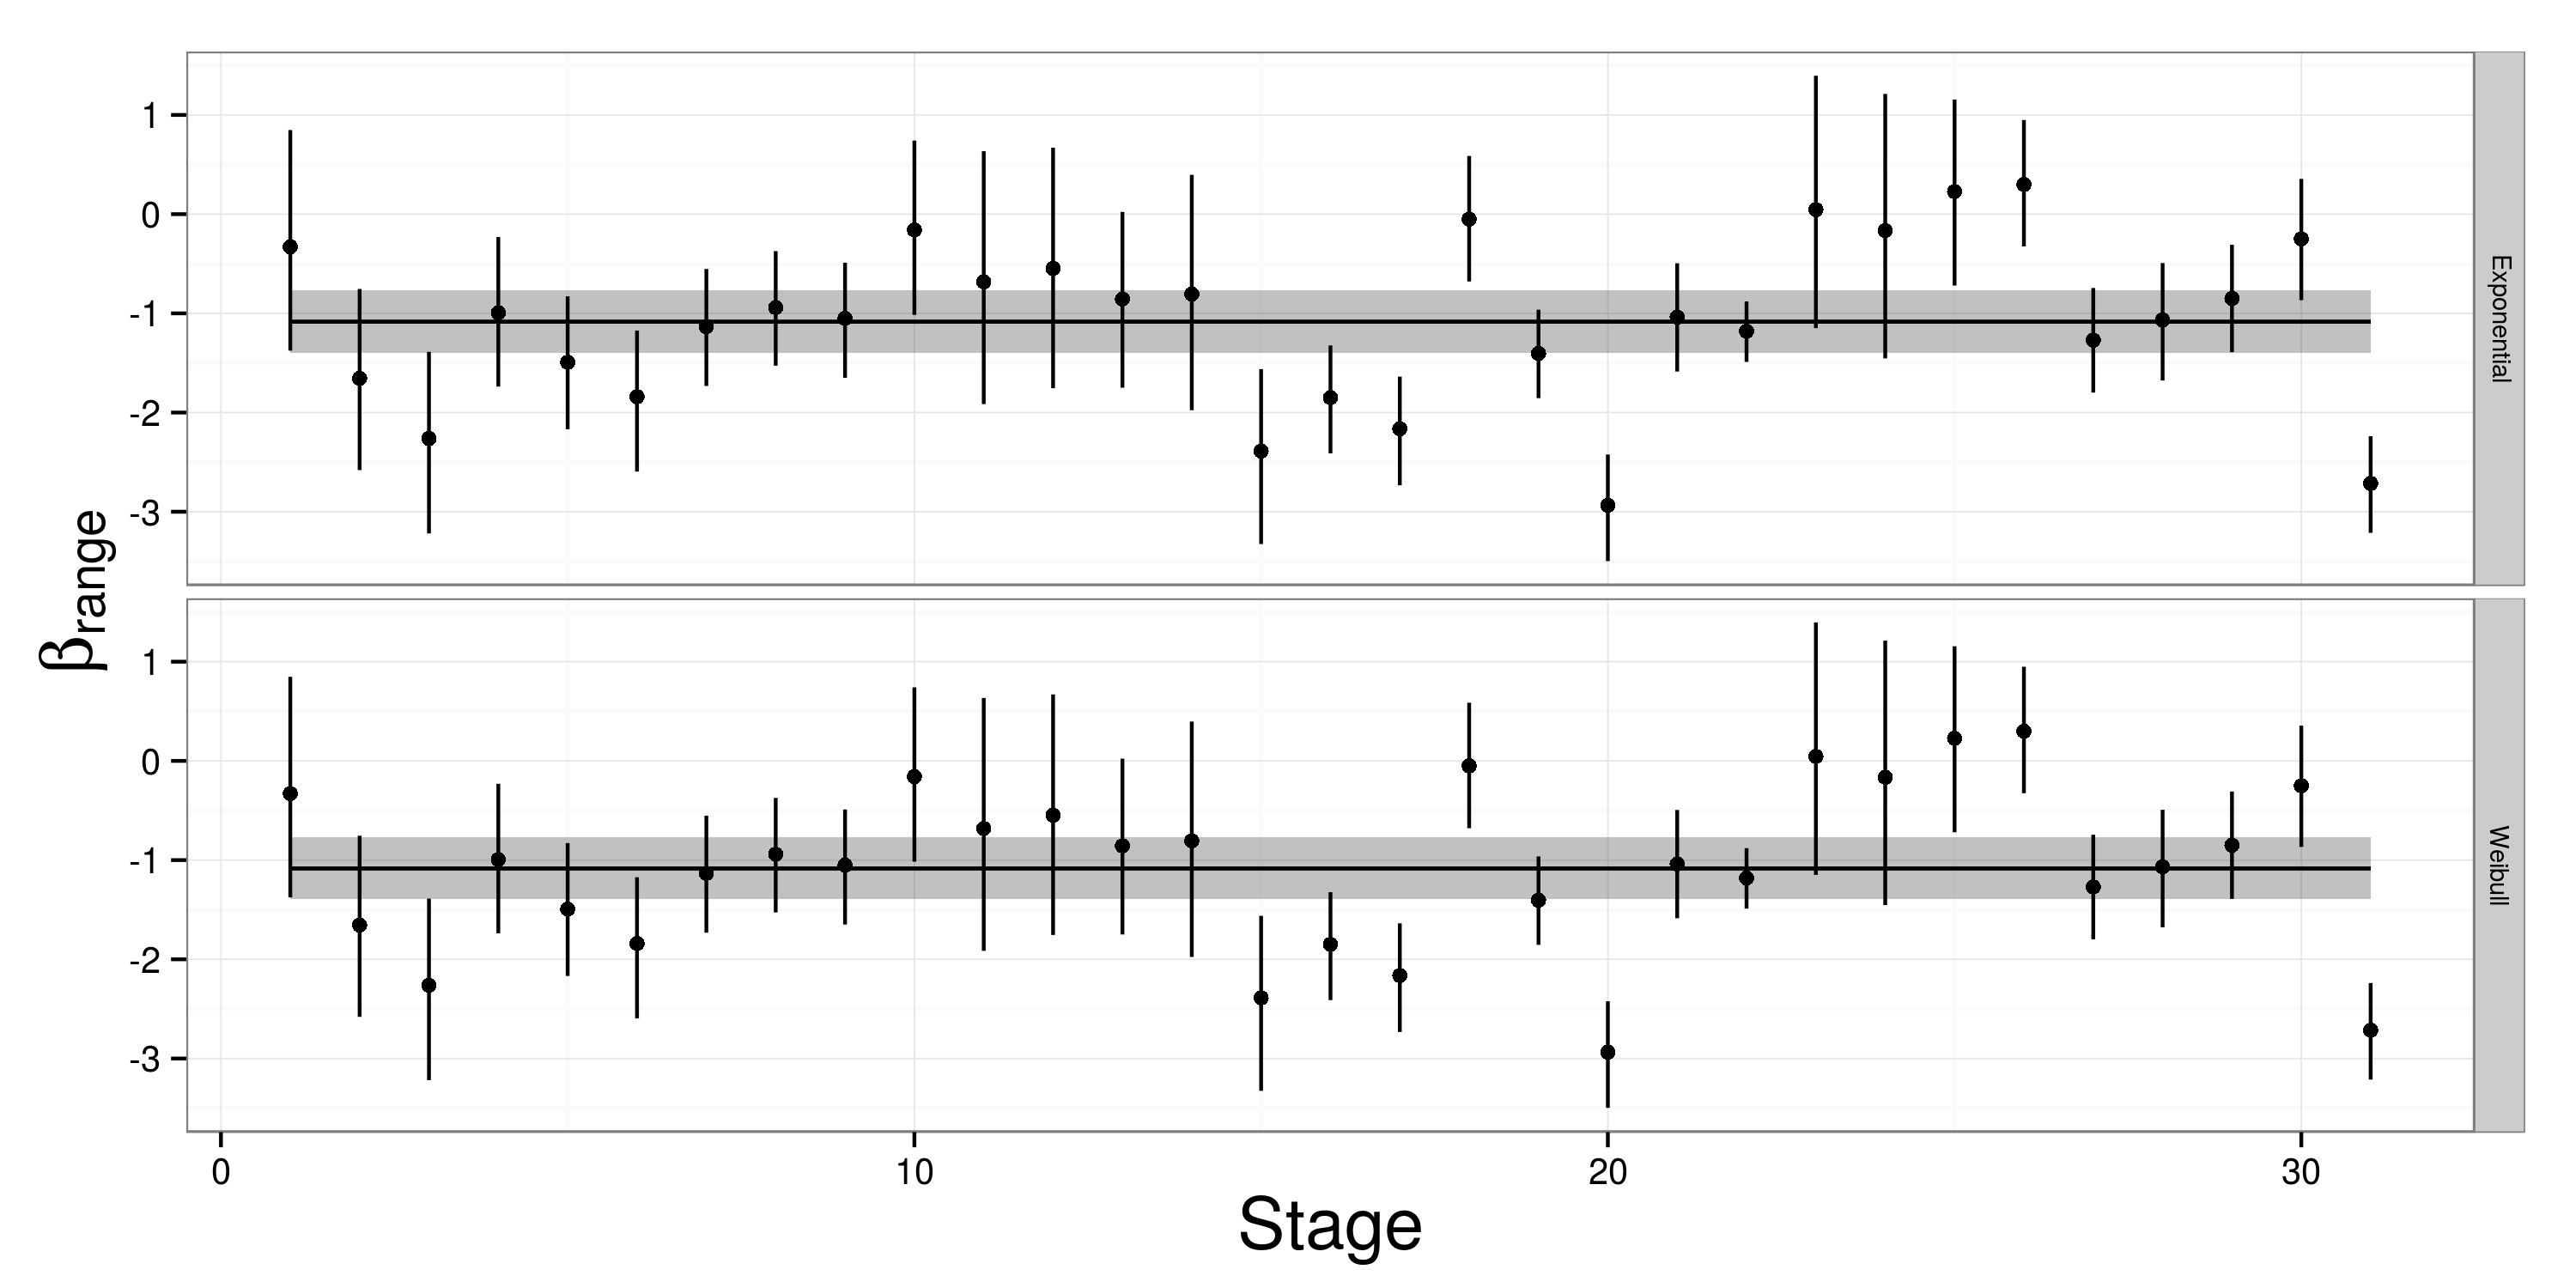
\includegraphics[width = \textwidth,keepaspectratio=true]{figure/range_cohort}
    \label{fig:cohort_range}
  \end{subfigure}
  \caption{Comparison of cohort-specific estimates of \(\beta_{0}\) presented along with the estimate for the overall baseline extinction risk. Points correspond to the median of the cohort-specific estimate, along with 80\% credible intervals. The horizontal line is the median estimate of the overall baseline extinction risk along with 80\% credible intervals. Results are presented for the exponential (top) and Weibull (bottom) models. Comparison of cohort-specific estimates of the effect of geographic range on extinction risk \(\beta_{r}\) presented along with the estimate for the overall effect of geographic range. Points correspond to the median of the cohort-specific estimate, along with 80\% credible intervals. The horizontal line is the median estimate of the overall baseline extinction risk along with 80\% credible intervals. Results are presented for the exponential (top) and Weibull (bottom) models.}
  \label{fig:cohort_info}
\end{figure}


\begin{sidewaysfigure}[ht]
  \centering
  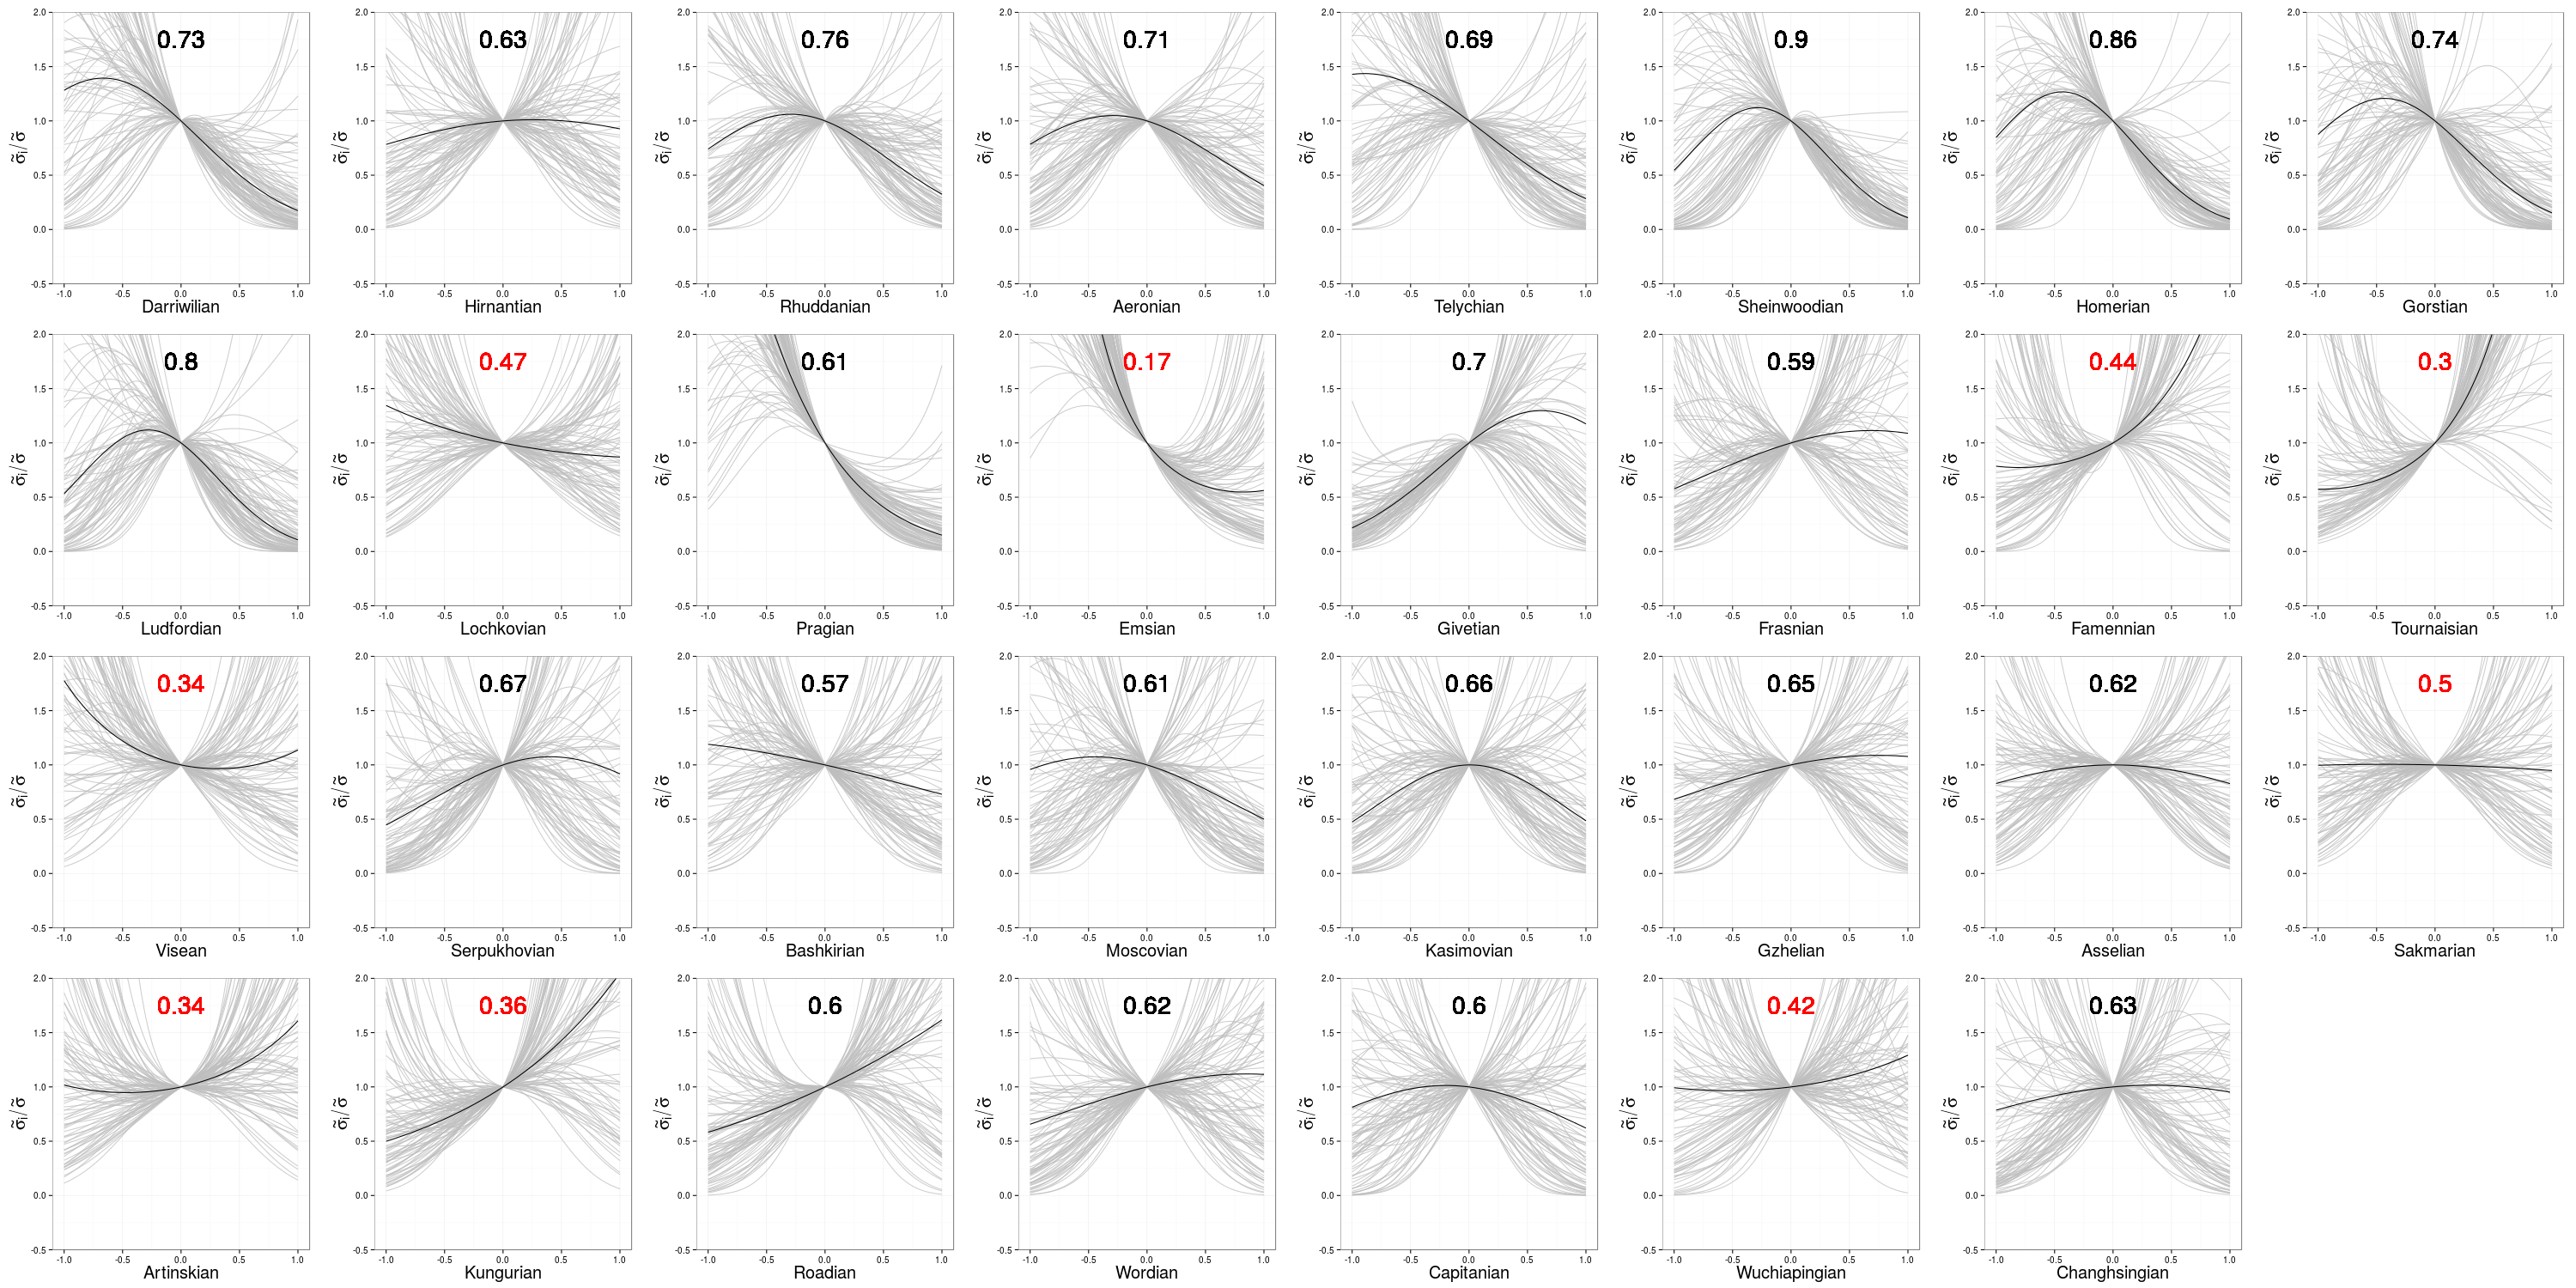
\includegraphics[height = 0.5\textheight,width=\textwidth,keepaspectratio=true]{figure/cohort_quads}
  \caption{Comparison of the cohort-specific estimates of \(f(v_{i})\) (Eq. \ref{eq:env}) for the 33 analyzed origination cohorts. The stage of origination is labeled on the x-axis of each panel. The oldest stage is in the upper left, while the youngest is in the lower left. The number in each panel corresponds to the posterior probability that \(f(v_{i})\) is concave down. Those that are highlighed in red have less than 51\% posterior predictive probability that \(f(v_{i})\) is concave down.}
  \label{fig:env_cohort}
\end{sidewaysfigure}

\begin{table}
  \centering
  \begin{tabular}{ l r r }
    \hline
    parameter & mean & standard deviation \\ 
    \hline
    \(\mu_{i}\) & -1.51 & 0.15 \\ 
    \(\mu_{r}\) & -1.38 & 0.14 \\ 
    \(\mu_{e}\) & -0.08 & 0.18 \\ 
    \(\mu_{e2}\) & 0.25 & 0.43 \\ 
    \(\mu_{m}\) & -0.09 & 0.09 \\ 
    \(\tau_{i}\) & 0.63 & 0.11 \\ 
    \(\tau_{r}\) & 0.48 & 0.12 \\ 
    \(\tau_{e}\) & 1.07 & 0.23 \\ 
    \(\tau_{e^{2}}\) & 1.88 & 0.66 \\ 
    \(\tau_{m}\) & 0.32 & 0.13 \\ 
    \hline
  \end{tabular}
  \caption{Group-level estimates of the intercept terms the effects of biological traits on brachiopod generic survival from equations \ref{eq:exp_total} and \ref{eq:wei_total}, presented as means and standard deviations. \(\mu\) values are the location parameters of the effects, while \(\tau\) values are the scale terms describing the variation between cohorts. The subscripts correspond to the following: \(i\) intercept, \(r\) geographic range, \(e\) environmental affinity, \(e^{2}\) environmental affinity squared, \(m\) body size.}
  \label{tab:param}
\end{table}

\clearpage

\appendix
\documentclass[12pt,letterpaper]{article}

\usepackage{amsmath, amsthm}
\usepackage{microtype, parskip}
\usepackage[comma,numbers,sort&compress]{natbib}
\usepackage{lineno}
\usepackage{docmute}
\usepackage{caption, subcaption, multirow, morefloats, rotating}
\usepackage{wrapfig}

\frenchspacing

\captionsetup[subfigure]{position = top, labelfont = bf, textfont = normalfont, singlelinecheck = off, justification = raggedright}

\begin{document}
\section{Uncertainty in environmental preference} \label{sec:uncer}
The calculation and inclusion of environmental affinity in the survival model is a statistical procedure that takes into account our uncertainty based on where fossils tend to occur. Because we cannot directly observe if a fossil taxon had occurrences restricted to only a single environment, instead we can only estimate its affinity with uncertainty. One advantage of using a Bayesian analytical approach is that both parameters and data are considered random samples from some underlying distribution, which means that is is possible to model the uncertainty in our covariates of interest \citep{Gelman2013d}. My approach is conceptually similar to \citet{Simpson2009} but instead of obtaining a single point estimate, an entire posterior distribution is estimated.

The first step is to determine the probability \(\theta\) at which genus \(i\) occurs in an epicontinental settings based on its own pattern of occurrences. Define \(e_{i}\) as the number of occurrences of genus \(i\) in an epicontiental sea and \(o_{i}\) as the number of occurrences of genus \(i\) not in an epicontinental sea (e.g. open ocean). Because the value of interest is the probability of occurring in an epicontinental environment, given the observed fossil record, I assume that probability follows a binomial distribution. We can then define our sampling statement as
\begin{equation}
  e_{i} \sim \mathrm{Binomial}(e_{i} + o_{i}, \theta_{i}).
  \label{eq:epi_lik}
\end{equation}
I used a flat prior for \(\theta_{i}\) defined as \(\theta_{i} \sim \mathrm{Beta}(1, 1)\). Because the beta distribution is the conjugate prior for the binomial distribution, the posterior is easy to compute in closed form. The posterior probability of \(\theta\) is then 
\begin{equation}
  \theta_{i} \sim \mathrm{Beta}(e_{i} + 1, o_{i} + 1)
  \label{eq:epi_post}
\end{equation}

It is extremely important, however, to take into account the overall environmental occurrence probability of all other genera present at the same time as genus \(i\). This is incorporated as an additional probability \(\Theta\). Define \(E_{i}\) as the total number of other fossil occurrences (exceptfor genus \(i\)) in epicontinental seas during stages where \(i\) occurs and \(O_{i}\) as the number of other fossil occurrences not on epicontinental seas. We can then define the sampling statement as
\begin{equation}
  E_{i} \sim \mathrm{Binomial}(E_{i} + O_{i}, \Theta_{i}).
  \label{eq:bck_lik}
\end{equation}
Again, I used a flat prior of \(\Theta_{i}\) defined as \(\Theta_{i} \sim \mathrm{Beta}(1, 1)\). The posterior of \(\Theta\) is then simply defined as

\begin{equation}
  \Theta_{i} \sim \mathrm{Beta}(E_{i} + 1, O_{i} + 1)
  \label{eq:bck_post}
\end{equation}

I then define the environmental affinity of genus \(i\) as \(v_{i} = \theta_{i} - \Theta_{i}\). \(v_{i}\) is a value that can range between -1 and 1, where negative values indicate that genus \(i\) tends to occur more frequently in open ocean environments than background while positive values indicate that genus \(i\) tends to occur in epicontiental environments.

While this approach is noticeably more complicated than previous ones \citep{Foote2006,Miller2001,Simpson2009,Kiessling2007a} there are some important benefits to both using a continuous measure of affinity as well directly modeling our uncertainty. In order to show some of these benefits, I performed a simulation analysis of how modal/maximum \textit{a posteriori} (MAP) estimates versus full posterior estimates.

In this simulation, I first defined the ``background'' epicontinental occurrence \(\theta_{b}\) as 0.50 with a small amount of noise. This was represented as a beta distribution 

\begin{equation}
  \Theta_{b} = \mathrm{Beta}(\alpha = 2500, \beta = 2500). 
  \label{eq:bck_sim}
\end{equation}
This choice of parameters for the distribution reflects the average number of background occurrences for either epicontinental or open ocean environments per genus.

Using this background occurrence ratio, I randomly generated the occurrence patterns of 1000 simulated taxa. This was done at multiple sample sizes (1, 2, 3, 4, 5, 10, 25, 50, 100) in order to demonstrate the effects of increasing sample size on the confidence of environmental affinity. For each simulated taxon I calculated the full posterior distribution while assuming a flat Beta prior (\(\mathrm{Beta}(1, 1)\)). Using the full posterior I calculated the MAP probability of occurring in epicontinental environments. The environmental affinity was calculated for each of the simulated taxa using both the full posterior and the MAP estimate. In this toy example, environmental affinity can range between -0.5 and 0.5.

As should be expected, as sample size increases the distribution of MAP estimates converge on the true value (Fig. \ref{fig:env_mode}). For taxa with less than 10 occurrences, the MAP estimate is biased towards extreme values. Note that the mode of the beta distribution is not defined for situations where there were 0 draws of one of the environmental conditions. Instead, the vertical line is based entirely on the observed occurrences which are technically the modal estimates because they are the most frequently occurring/highest density.

In contrast, we can compare the true occurrence probability distribution versus the posterior estimate for a given sample (Fig. \ref{fig:env_post}). When sample sizes are low, posterior estimates are flat and represent a compromise between the likelihood and the flat prior (Eq. \ref{eq:epi_post}). Because of this, estimates from small sizes are less likely to be overly biased towards the extremes. This is further emphasized by inspection of the estimates of environmental affinity for the simulated taxa (Fig. \ref{fig:env_diff}). Posterior estimates from simulated taxa with small sample size have a much broader distribution that both allows for the extreme observation but still captures the ``true'' value (0). 


By defining environmental preference as the difference in full posterior estimates of occurrence probability, it is possible to include taxa with low sample sizes that are normal discarded \citep{Foote2006,Miller2001,Simpson2009,Kiessling2007a}. Additionally, 55+\% of observed Paleozoic brachiopod genera have less than 10 occurrences which is the range of sample sizes where MAP (or ML) estimates would be potentially most biased. This is preferable to finding the difference between the MAP estimates (blue line; Fig. \ref{fig:env_diff}).

% behavior of MAP estimates
%   as sample size increases, converge on true (10+)
% behavior of posterior
%   compromise between likelihood of data occurrences and (flat) prior
%   really important for small sample sizes
%   at 10+ makes no difference anymore
%   this is also kind obvious from the estimates of \(v\)
% how many taxa have less than 10 occurrences? \approx 55\%

\begin{figure}[ht]
  \centering
  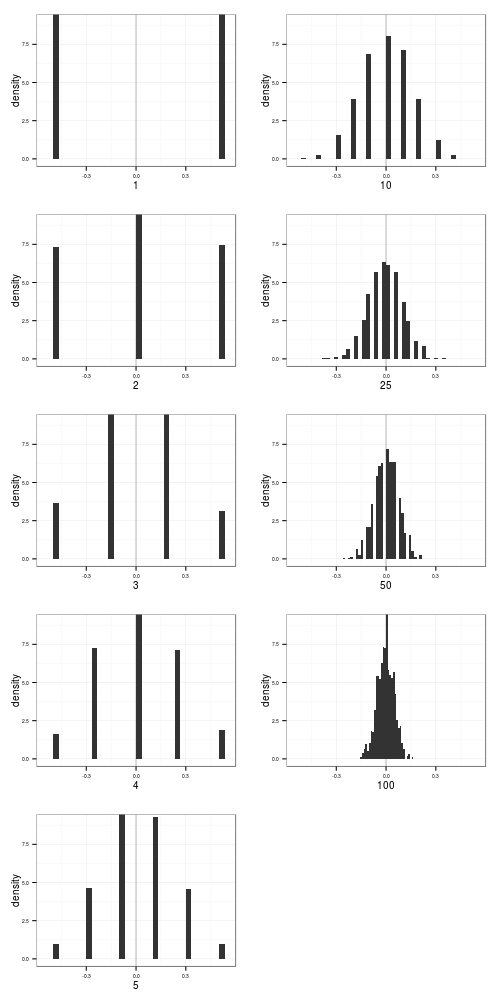
\includegraphics[height = \textheight,width=\textwidth,keepaspectratio=true]{figure/env_mode_dist}
  \caption{Histograms of the distributions of from the beta distribution defined in Eq. \ref{eq:bck_sim}. As to be expected, as sample size increases the draws better resemble the underlying true distribution. Sample size is indicated as the label of the x-axis, increasing in column major order.}
  \label{fig:env_mode}
\end{figure}

\begin{figure}[ht]
  \centering
  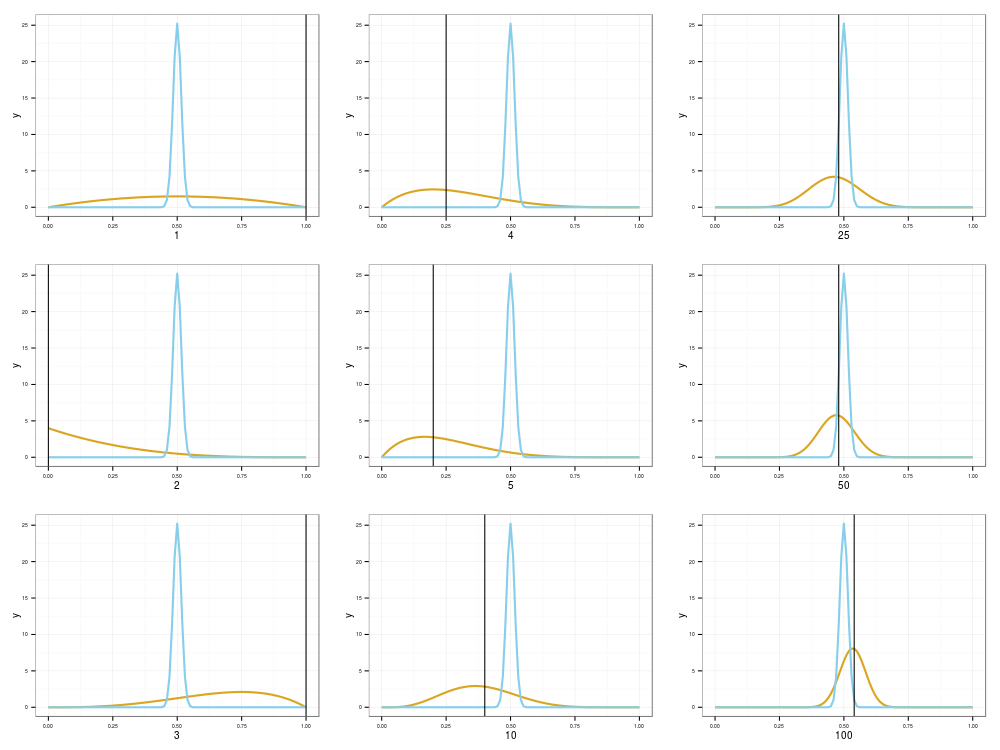
\includegraphics[height = \textheight,width=\textwidth,keepaspectratio=true]{figure/env_post_inspect}
  \caption{Comparisons of the underlying distribution (blue) to posterior estimates based on increasing sample size (gold). Each posterior estimate is represented for only a single realization of draws, each with sample size indicated as the x-axis label (increasing in column major order). Black vertical lines correspond to the MAP estimate of the simulated taxon's affinity. This stands in contrast to the posterior distribution of expected affinity in gold.}
  \label{fig:env_post}
\end{figure}

\begin{figure}[ht]
  \centering
  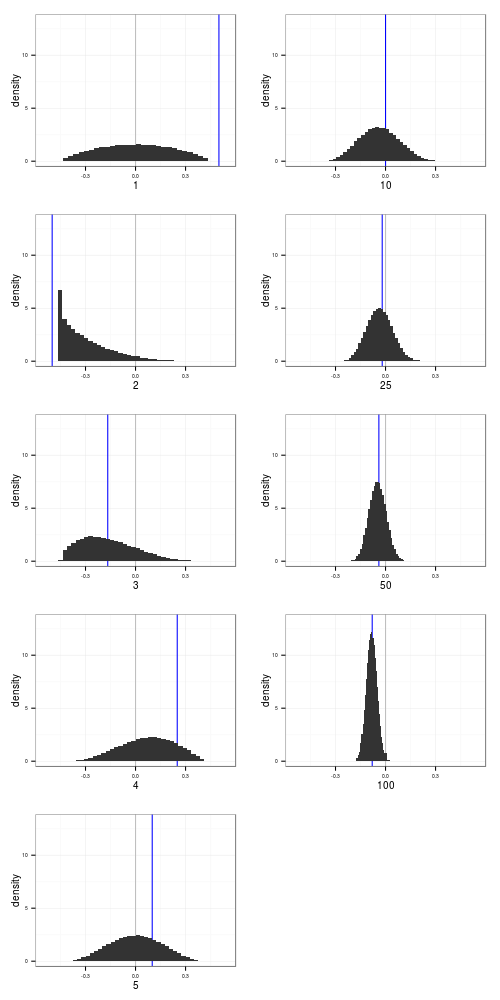
\includegraphics[height = \textheight,width=\textwidth,keepaspectratio=true]{figure/env_diff}
  \caption{Histograms of the difference in the underlying occurrence distribution and the posterior distribution estimates from the previous graph (Fig. \ref{fig:env_post}). The ``true'' value is included in all distributions of environmental affinities. Each affinity estimate is represented for only a single realization of draws, each with sample size indicated as the x-axis label (increasing in column major order). Blue vertical lines correspond to the difference in MAP estimates between the underlying distribution and the simulated taxon's draws. This stands in contrast to the distribution of the differences between the simulated taxon and background.}
  \label{fig:env_diff}
\end{figure}

\section{Survival model} \label{sec:survival}

The simplest model of genus duration includes no covariate or structural information. Define \(y_{i}\) as the duration in stages of genus \(i\), where \(i = 1, \dots, n\) and \(n\) is the number of observed genera. These two models are them simply defined as
\begin{equation}
  \begin{aligned}
    y_{i} &\sim \mathrm{Exponential}(\lambda) \\
    y_{i} &\sim \mathrm{Weibull}(\alpha, \sigma).
  \end{aligned}
  \label{eq:simple}
\end{equation}
\(\lambda, \alpha, \text{and} \sigma\) are all defined for all positive reals. Note that \(\lambda\) is a ``rate'' or inverse-scale while \(\sigma\) is a scale parameter, meaning that \(\frac{1}{\lambda} = \sigma\).

These simple models can then be expanded to include covariate information as predictors by reparameterizing \(\lambda\) or \(\sigma\) as a regression \citep{Klein2003}. Each of the covariates of interest is given its own regression coefficient (e.g. \(\beta_{r}\)) along with an intercept term \(\beta_{0}\). There are some additional complications to the parameterization of \(\sigma\) associated with the inclusion of \(\alpha\) as well as for interpretability \citep{Klein2003}. Both of these are then written as
\begin{equation}
  \begin{aligned}
    \lambda_{i} &= \exp(\beta_{0} + \beta_{r} r_{i} + \beta_{v} v_{i} + \beta_{v^{2}} v_{i}^{2} + \beta_{m} m_{i}) \\
    \sigma_{i} &= \exp\left(\frac{-(\beta_{0} + \beta_{r} r_{i} + \beta_{v} v_{i} + \beta_{v^{2}} v_{i}^{2} + \beta_{m} m_{i})}{\alpha}\right).
  \end{aligned}
  \label{eq:regression}
\end{equation}
The quadratic term for environmental affinity \(v\) is to allow for the possible nonlinear relationship between environmental affinity and extinction risk.

The models which incorporate both equations \ref{eq:simple} and \ref{eq:regression} can then be further expanded to allow all of the \(\beta\) coefficients, including \(\beta_{0}\), to vary with origination cohort while also modeling their covariance and correlation. This is called a varying-intercepts, varying-slopes model \citep{Gelman2007}. It is much easier to represent and explain how this is parameterized using matrix notation. First, define \(\mathbf{B}\) as \(k \times J\) matrix of the \(k\) coefficients including the intercept term (\(k = 5\)) for each of the \(J\) cohorts. Second, define \(\mathbf{X}\) as a \(n \times k\) matrix where each column is one of the covariates of interest. Importantly, \(\mathbf{X}\) includes a columns of all 1s which correspond to the constant term \(\beta_{0}\). Third, define \(j[i]\) as the origination cohort of genus \(i\), where \(j = 1, \dots, J\) and \(J\) is the total number of observed cohorts. We then rewrite \(\lambda\) and \(\sigma\) of equation \ref{eq:regression} in matrix notation as
\begin{equation}
  \begin{aligned}
    \lambda_{i} &= \exp(\mathbf{X}_{i} B_{j[i]}) \\
    \sigma_{i} &= \exp\left(\frac{-(\mathbf{X}_{i} B_{j[i]})}{\alpha}\right). 
  \end{aligned}
  \label{eq:multivariate}
\end{equation}

Because \(B\) is a matrix, I use a multivariate normal prior with unknown vector of means \(\mu\) and covariance matrix \(\Sigma\). This is written as 
\begin{equation}
  B \sim \mathrm{MVN}(\vec{\mu}, \Sigma)
  \label{eq:beta_prior}
\end{equation}
where \(\vec{\mu}\) is length \(k\) vector representing the overall mean of the distributions of \(\beta\) coefficients. \(\Sigma\) is a \(k \times k\) covariance matrix of the \(\beta\) coefficients.

What remains is assigning priors the elements of \(\vec{\mu}\) and the covariance matrix \(\Sigma\). All elements of \(\vec{\mu}\) except for \(\mu_{r}\) were given horseshoe priors \citep{Carvalho2010,Carvalho2009} while \(\mu_{r}\) was given an informative normal prior (\(\mu_{r} \sim \mathcal{N}(-1, 1)\). Horseshoe priors are a strong regularizing priors with effectively infinite density at 0 and heavy, Cauchy-like tails \citep{Carvalho2010,Carvalho2009} which allow weakly inferred effects to be strongly drawn towards 0 while truly strong effects can remain large. The horseshoe prior consists of a normal distribution with scale term that is the product between a global shrinkage parameter \(\nu\) and a locak shrinkage parameter \(\psi\) unique to each of the parameters of interest. These parameters are themselves given half-Cauchy priors (Eq. \ref{eq:exp_total} and \ref{eq:wei_total}).

The prior for \(\Sigma\) is a bit more complicated due to its multivariate nature. Following the \citet{stan-manual:2014}, I modeled the scale terms separate from the correlation structure of the coefficients. This is possible because of the relationship between a covariance and a correlation matrix, defined as 
\begin{equation}
  \Sigma_{B} = \text{Diag}(\vec{\tau}) \Omega \text{Diag}(\vec{\tau})
  \label{eq:covcor}
\end{equation}
where \(\vec{\tau}\) is a length \(k\) vector of variances and Diag(\(\tau\)) is a diagonal matrix.

I used a LKJ prior distribution for correlation matrix \(\Omega\) as recommended by \citet{stan-manual:2014}. The LKJ distribution is a single parameter multivariate distribution where values of the parameter \(\eta\) greater than 1 concentrate density at the unit correlation matrix, which corresponds to no correlation between the \(\beta\) coefficients. The scale parameters, \(\vec{\tau}\), are given weakly informative half-Cauchy (C\(^{+}\)) priors following \citet{Gelman2006a}.



\section{Censored observations} \label{sec:cen}
A key aspect of survival analysis is the inclusion of censored, or incompletely observed, data points \citep{Ibrahim2001,Klein2003}. The two classes of censored observations encountered in this study were right and left censored observations. Right censored genera are those that did not go extinct during the window of observation, or genera that are still extant. Left censored observations are those taxa for which we know only an upper limit on their duration.

In the context of this study, I considered all genera that had a duration of only one geologic stage to be left censored as we do not have a finer degree of resolution. 

The key function for modeling censored observations is the survival function, or \(S(t)\). \(S(t)\) corresponds to the probability that a genus having existed for \(t\) stages will not have gone extinct while \(h(t)\) corresponds to the instantaneous extinction rate at taxon age \(t\) \cite{Klein2003}. For an exponential model, \(S(t)\) is defined as
\begin{equation}
  S(t) = \exp(-\lambda t),
  \label{eq:exp_surv}
\end{equation}
and for the Weibull distribution \(S(t)\) is defined as
\begin{equation}
  S(t) = \exp\left(-\left(\frac{t}{\sigma}\right)^{\alpha}\right).
  \label{eq:wei_surv}
\end{equation}
\(S(t)\) is equivalent to the complementary cumulative distribution function, \(1 - F(t)\) \citep{Klein2003}. 

For right censored observations, instead of calculating the likelihood as normal (Eq. \ref{eq:multivariate}) the likelihood of an observation is evaluated using \(S(t)\). Conceptually, this approach calculates the likelihood of observing a taxon that existed for at least that long. For left censored data, instead the likelihood is calculated using \(1 - S(t)\) which corresponds to the likelihood of observing a taxon that existed no longer than \(t\).

The full likelihood statements incorporating fully observed, right censored, and left censored observations are then
\begin{equation}
  \begin{aligned}
    \mathcal{L} &\propto \prod_{i \in C} \mathrm{Exponential}(y_{i} | \lambda) \prod_{j \in R} S(y_{j} | \lambda) \prod_{k \in L} \left(1 - S(y_{k} | \lambda)\right) \\
    \mathcal{L} &\propto \prod_{i \in C} \mathrm{Weibull}(y_{i} | \alpha, \sigma) \prod_{j \in R} S(y_{j} | \alpha, \sigma) \prod_{k \in L} \left(1 - S(y_{k} | \alpha, \sigma)\right)
  \end{aligned}
  \label{eq:censored_likelihood}
\end{equation}
where \(C\) is the set of all fully observed taxa, \(R\) the set of all right censored taxa, and \(L\) the set of all left-censored taxa.


\section{Widely applicable information criterion} \label{sec:waic}
WAIC can be considered a fully Bayesian alternative to the Akaike information criterion, where WAIC acts as an approximation of leave-one-out cross-validation which acts as a measure of out-of-sample predictive accuracy \citep{Gelman2013d}. WAIC is calculated starting with the log pointwise posterior predictive density calculated as
\begin{equation}
  \mathrm{lppd} = \sum_{i = 1}^{n} \log \left(\frac{1}{S} \sum_{s = 1}^{S} p(y_{i}|\Theta^{S})\right),
  \label{eq:lppd}
\end{equation}
where \(n\) is sample size, \(S\) is the number posterior simulation draws, and \(\Theta\) represents all of the estimated parameters of the model. This is similar to calculating the likelihood of each observation given the entire posterior. A correction for the effective number of parameters is then added to lppd to adjust for overfitting. The effective number of parameters is calculated, following the recommendations of \citet{Gelman2013d}, as
\begin{equation}
  p_{\mathrm{WAIC}} = \sum_{i = 1}^{n} V_{s = 1}^{S} (\log p(y_{i}|\Theta^{S})).
  \label{eq:pwaic}
\end{equation}
where \(V\) is the sample posterior variance of the log predictive density for each data point.

Given both equations \ref{eq:lppd} and \ref{eq:pwaic}, WAIC is then calculated
\begin{equation}
  \mathrm{WAIC} = \mathrm{lppd} - p_{\mathrm{WAIC}}.
  \label{eq:waic}
\end{equation}
When comparing two or more models, lower WAIC values indicate better out-of-sample predictive accuracy. Importantly, WAIC is just one way of comparing models. When combined with posterior predictive checks it is possible to get a more complete understanding of a model's fit to the data.

\end{document}



\end{document}

